\subsection{Analysis Overview}
\label{subsec:ana_overview}
The analysis relies on Monte Carlo events that are fully simulated using the ILD detector model \url{ ILD_l5_o1_v02 } with iLCSoft version v02-00-02 and includes a complete standard model background for final states with 2,4, and 6 fermions as well standard model Higgs production.  A center of mass energy of 500 GeV and longitudinally-polarized beams in various operating scenarios are considered. The Monte Carlo events are generated for $100\%$ polarized beams, that is, either all left or right handed. Events are weighted in order to obtain realistic cases of partial polarizations for possible running scenarios which are shown in Table \ref{tab:beamscenario}.

\begin{table}

\caption{Possible running configurations with partial beam polarizations ($P_{e^-},P_{e^+}$) and integrated luminiosity \cite{ilcop} }
\label{tab:beamscenario}
\begin{tabular}{|c|c|c|c|c|}
\hline 
Pol. &(-0.8,+0.3) & (+0.8,-0.3) & (-0.8,-0.3) & (+0.8,+0.3) \\ 
\hline 
$\int$ Lum. [fb$^{-1}$] & 1600 & 1600 & 400 & 400 \\ 
\hline 
\end{tabular} 

\end{table}
 The partial polarizations $P_{e^-} \, \, P_{e^+}$  can be represented by the fraction of the beam which is either left or right handed
 \begin{equation}
 \begin{split}
f_R^{e^-} + f_L^{e^-} = 1 \, \, \, \, \, \, f_R^{e^-} = \frac{1}{2}(1 + P_{e^-}) \\
f_R^{e^+} + f_L^{e^+} = 1 \, \, \, \, \, \, f_R^{e^+} = \frac{1}{2}(1 + P_{e^+})
\end{split}
 \end{equation}
where the beam fraction $f$ is denoted with the polarization subscript and respective beam superscript. For a particular scenario like $(P_{e^-}, P_{e^+}) = (-0.8, +0.3)$ the -0.8 represents an electron beam with $90\% $ left handed electrons mixed with $10\% $ right handed electrons and a positron beam with $65\%$ right handed positrons mixed with $35\%$ left handed positrons. The weight $\omega$ for a specific event with particular initial state helicities is given by (with example partial polarizations (-0.8,+0.3) ):
 \begin{equation}
 \begin{split} 
 \omega_{LR} = f_L^{e^-}f_R^{e^+} = 0.9 \times 0.65 = 0.585 \\
 \omega_{RL} = f_R^{e^-}f_L^{e^+} = 0.1 \times 0.35 = 0.035 \\
 \omega_{LL} = f_L^{e^-}f_L^{e^+} = 0.9 \times 0.35 = 0.315 \\
 \omega_{LR} = f_R^{e^-}f_R^{e^+} = 0.1 \times 0.65 = 0.065 
 \end{split}
 \end{equation} 

The analysis workflow for semileptonic WW has three distinct stages, the lepton identification and selection, pile-up rejection in the hadronic system, and event selection against against full standard model backgrounds. The analysis is performed with the  running scenario that creates the most dominant WW production mode (-0.8,+0.3). 


\subsection{Lepton Identification}
\label{subsec:Lepton_ID}
The approach towards the identification of leptons relies on treating leptons universally. The easiest lepton to identify is the muon, which produces a single track along with hits in the muon detector. The electron also produces a track in the TPC but is often accompanied by photons via bremsstrahlung radiation. The tau is the most difficult lepton to identify due to its decay into multiple charged and neutral particles. To accommodate all types lepton signature, a cone based approach is used to either capture single tracks or collimated jets with low track multiplicity. The lepton finding cone is based on TauFinder \cite{taufinder} designed for the Compact Linear Collider(CLIC). TauFinder consists of two major structures, a search cone containing the particles that belong to the lepton candidate and an isolation cone whose purpose is to reject a lepton candidate if the search cone is not well-isolated from other particles. The acceptance criteria for cone consists of these parameters:
\begin{itemize}
\item Search cone angle $\alpha$ - The opening (half) angle of the search cone for the lepton jet [rad]
\item Isolation cone angle $\beta$ - The outer isolation cone angle w.r.t to the search cone [rad]
\item Isolation energy - The total energy allowed within the isolation cone region [GeV]
\item Invariant Mass - The upper limit on the lepton candidate mass [GeV]
\item Track multiplicity - The allowed number of tracks in a lepton candidate
\item Minimum $P_t$ seed - the minimum transverse momentum of a track that seeds a lepton candidate [GeV] 
\end{itemize}
An example of the cone and parameters are shown in Figure \ref{fig:cone}. Additional requirements are imposed on all of the reconstructed Particle Flow Objects(PFOs) in the event in order to suppress pile-up particles being included in the lepton jet.
\begin{itemize}
\item $P_t > 0.2$ GeV
\item $|cos\theta| < 0.99$
\end{itemize}
The formation of a lepton candidate follows three steps (1) candidate construction, (2) candidate merging, and (3) isolation testing.
The first step starts with seed tracks that are sorted by energy in descending order. Any track or neutral particle that falls within the search cone of the lepton candidate is added to the lepton candidate. For each newly added particle the energy and momentum is updated for the lepton candidate. Each candidate has a unique set of particles. Lepton candidates are continually formed until the seed tracks exhausted. When there are no more candidates to be created, the candidates are subjected to part of the acceptance criteria: the lepton jet mass is required to be below upper mass limit (2 GeV) and the number of charged tracks within the lepton candidate is non-zero and less than or equal to 4. If a lepton jet violates any acceptance conditions it is deleted. The next step in the process is merging. If two lepton candidates fall within each others search cones, the candidates are merged. If the mass or track multiplicity conditions are violated, both lepton candidates are deleted.  All  candidates that survive merging are subjected to the isolation testing. For each candidate, the sum of energy of all the particles that fall inside the isolation cone is computed. If the total energy inside the isolation cone is greater than the maximum allowed energy inside the isolation cone the lepton candidate is deleted.\\
\quad \quad \\
The universal lepton treatment is not conducive to a one size fits all approach to lepton ID due to the abundance of different lepton signatures. To accomodate for variations between lepton signatures, the acceptance criteria for leptons is optimized according to lepton flavor and $\tau$ decay topology. The categories created are:\\

\begin{minipage}[h]{0.48\textwidth}
\centering
\begin{itemize}
\item Prompt $\mu$
\item Prompt $e$
\item $\tau \rightarrow \mu \bar{\nu_{\mu}} \nu_{\tau} $
\item $\tau \rightarrow e \bar{\nu_{e}} \nu_{\tau} $
\item $\tau \rightarrow$ hadrons (1-prong)
\item $\tau \rightarrow$ hadrons (3-prong)
\end{itemize}
\end{minipage}\hfill
\begin{minipage}[h]{0.48\textwidth}
\label{fig:cone}
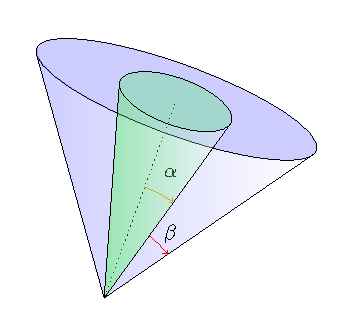
\includegraphics[width=0.6\textwidth]{cone.pdf}
\captionof{figure}{Illustration of possible lepton candidate cone with search cone angle $\alpha$ and isolation cone angle $\beta$. The search cone is shown in green and the isolation cone is the surrounding blue cone.}

\end{minipage}\\

The Prompt categories refer to events in which the leptonic W decays directly to either a muon or electron and associated neutrino. The tau categories address the various dominant decay topologies of the tau lepton. For each category, the optimal lepton acceptance criteria is calculated with respect to the events that match the desired topology. The optimal acceptance criteria is the set of parameters that maximally identify lepton candidates that originate from true leptons and minimize the fake lepton candidates that originate from hadronic jets. To find this set of parameters, a scan over a 3D space is performed using the search cone-$\alpha$, isolation cone-$\beta$, and isolation energy-$E_{iso}$. The invariant mass is held at a fixed 2 GeV for simplicity.
Two uncorrelated push-pull parameters are defined to find the optimal working point in the lepton finding space. The first is related to correctly identifying jets originating from true leptons. This is denoted as the efficiency of reconstructing a true lepton $\epsilon_T$. The second optimization parameter is denoted as $P_F$, the probability of a fake lepton jet arising from a single hadronic jet.  
\begin{equation}
\label{eq:et}
\epsilon_T = N_{match}/N_{Stotal}
\end{equation}
\begin{equation}
\begin{split}
\label{eq:pf}
P_F = 1-(1-\epsilon_F)^{\frac{1}{4}} \\
\epsilon_F = N_{fake}/N_{Btotal}
\end{split}
\end{equation}
The true lepton reconstruction efficiency is maximized with the signal sample $WW\rightarrow q\bar{q}\ell\nu$. The denominator represents the total, category specific, number of events which contain three generator visible fermions. The true $q\bar{q}\ell$ fermions are required to fall within the acceptance range $|cos\theta| < 0.99$. $N_{match}$ is the number of signal sample events in which a lepton candidate is reconstructed and can be matched to the true lepton, such that the opening angle between the reconstructed lepton and the true lepton are less than 0.1 radians. The distribution of opening angles is shown if Figure \ref{fig:taupsi}. In the case that a reconstructed lepton is being matched to a true tau, the matching angle formed between the reconstructed lepton and the vector sum of the visible generator components of the tau decay. The visible components of the tau decay consist of the direct decay products whereas photons from final state radiation are excluded. The fake lepton probability $P_f$ is minimized using the background sample $WW\rightarrow q\bar{q}q\bar{q}$ and is a function of the fake lepton reconstruction efficiency $\epsilon_F$. The denominator for fake is also subjected to the same acceptance range $|cos\theta| < 0.99$ for all four fermions. The numerator is the total number of events  that contain at least one reconstructed fake lepton. The fake efficiency can be interpreted as the binomial probability of $r$-successes(lepton reconstructions) in 4 trials(hadronic jets). The probability of a single success in a single trial, $P_F$, can be directly derived from the binomial p.d.f using the fake efficiency $\epsilon_F$. The optimal parameters $\alpha$, $\beta$, $E_{iso}$ for each lepton category are extracted from max$[(1-P_F)\epsilon_T]$. The results for each category are shown in Table \ref{tab:taufinderopt}. 


\begin{figure}
\centering
    \begin{minipage}{0.48\textwidth}
        \centering

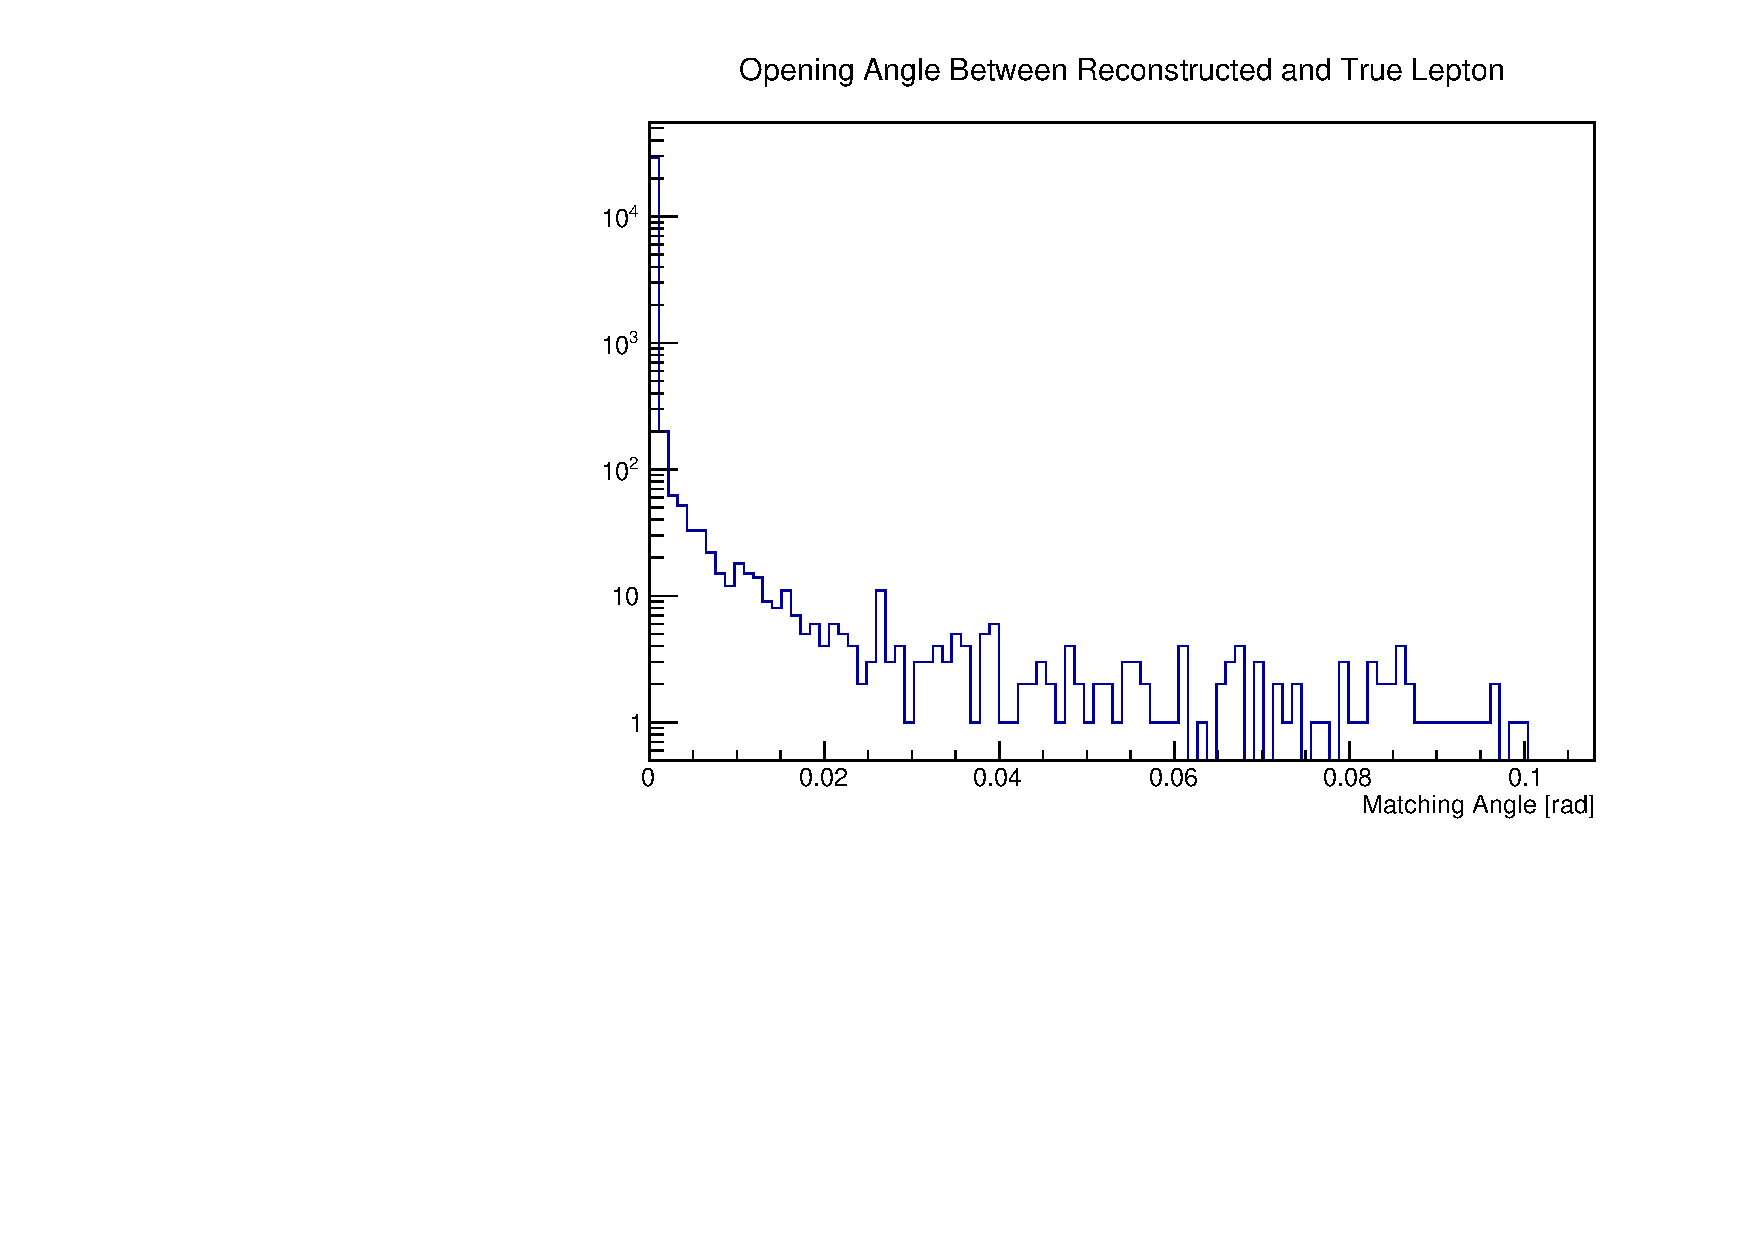
\includegraphics[width=0.9\textwidth]{matchingangle.pdf}
\caption{Distribution of opening angles between the closest reconstructed lepton candidate and the true muon from $WW \rightarrow q \bar{q} \mu \nu_\mu$. $99.4\%$ of events with a muon candidate are matched to truth.} 
\label{fig:taupsi}
\end{minipage}\hfill
    \begin{minipage}{0.48\textwidth}
        \centering

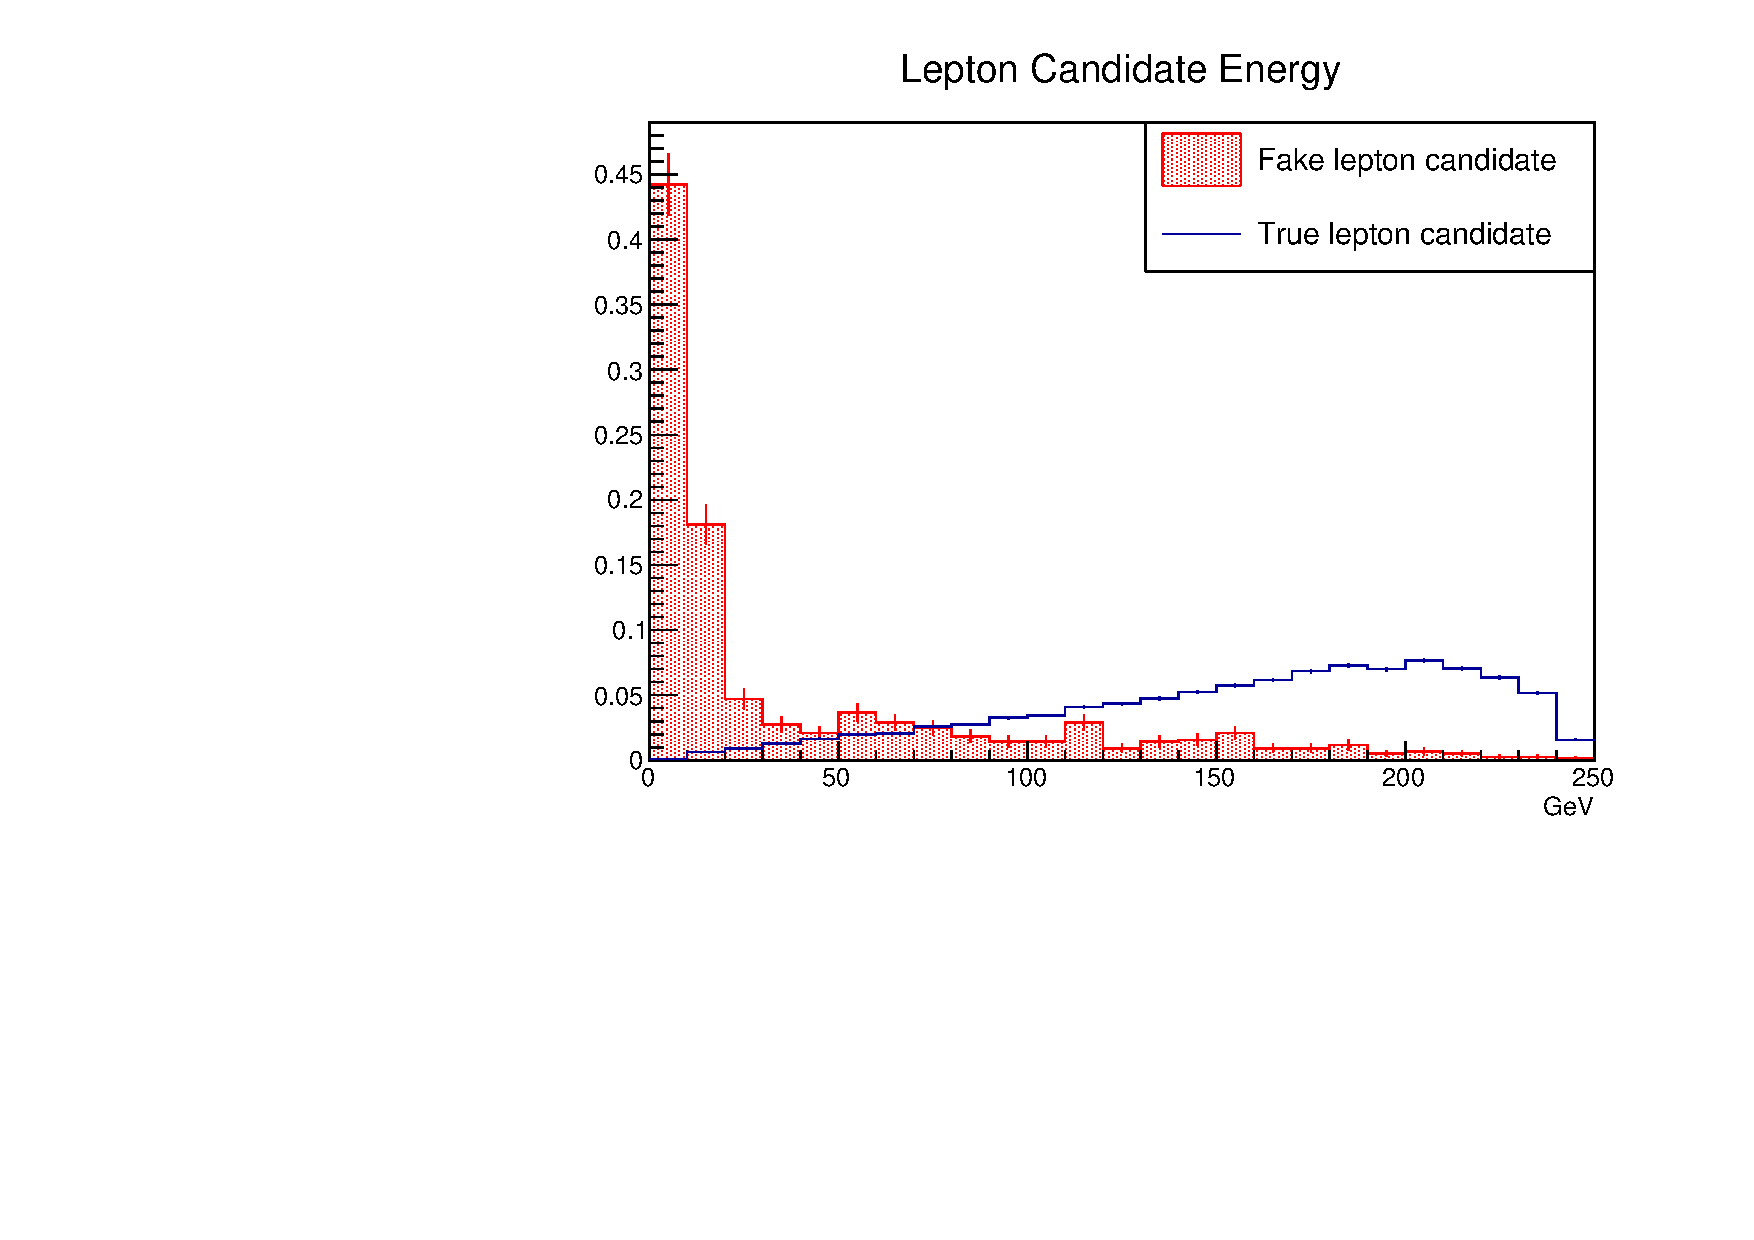
\includegraphics[width=0.9\textwidth]{candEnergy.pdf}
\caption{Energy distribution of lepton candidates matched to truth from $WW \rightarrow q \bar{q} \mu \nu_\mu $ and fake candidates from $ WW \rightarrow q\bar{q} q \bar{q}$ both normalized to unity.}
\label{fig:candE}
\end{minipage}
\end{figure}



\begin{table}

\begin{tabular}{|p{0.15\textwidth}|p{0.16\textwidth}p{0.16\textwidth}p{0.16\textwidth}p{0.1\textwidth}p{0.1\textwidth}p{0.1\textwidth}|}

\hline 
Channel & $n \, \, \text{Lep} \geq 1$ & $1-P_{F}$ & $\epsilon_T$ & SearchCone [rad] & Iso.Cone [rad] & Iso.E [GeV] \\ 
\hline 
Prompt $\mu$ & $0.955 \pm 0.003$ & $0.974 \pm 0.001$ & $0.949 \pm 0.003$ & 0.03 & 0.15 & 3.0 \\ 

Prompt $e$ & $0.920 \pm 0.003$ & $0.961 \pm 0.001$ & $0.904 \pm 0.003$ & 0.04 & 0.15 & 4.0 \\ 

Inclusive $\tau$ & $0.800 \pm 0.005$ & $0.943 \pm 0.001$ &  $0.770 \pm 0.006$ & 0.07 & 0.15 & 4.5 \\ 


 \hline
$\tau \rightarrow \nu \nu \mu$ & $0.815 \pm 0.012$ & $0.974 \pm 0.001$ & $0.801 \pm 0.013$ & 0.03 & 0.15 & 3.0 \\ 
 
$\tau \rightarrow \nu \nu e$ &  $0.800 \pm 0.012$ & $0.963 \pm 0.001$ &  $0.781 \pm 0.013$ & 0.05 & 0.15 & 3.5 \\ 
 
$\tau$ Had-1p & $0.744 \pm 0.009$ & $0.930 \pm 0.002$ & $0.707 \pm 0.009$ & 0.07 & 0.15 & 4.5 \\ 
 
$\tau$ Had-3p &  $0.756 \pm 0.015$ & $0.930 \pm 0.002$ & $0.710 \pm 0.016$ & 0.07 & 0.15 & 5.5  \\
\hline
\end{tabular} 
\caption{Optimization results using $100 \%$ LR $q\bar{q}\ell \nu$ and $q\bar{q} q\bar{q}$ samples. The $n \, \, \text{Lep} \geq 1$ column pertains to signal samples where at least one lepton candidate was found and is not subjected to the truth matching criteria of 0.1 radians. Results shown are the configurations that maximize $(1-P_F)\epsilon_T$ }
\label{tab:taufinderopt}
\end{table}

Since only one lepton is expected from signal, a single lepton candidate is selected as the candidate for the event. If multiple lepton jets are reconstructed then the lepton candidate with the highest energy is selected as the single candidate for the event. The energy distribution of true and fake leptons is shown in Figure \ref{fig:candE}. If the two highest energy lepton jets are of equal energy then the candidate selected will be the jet with the highest energy original seed track, due to seed track sorting.  Any additional lepton candidates not selected are treated as part of the hadronic system.


\subsection{Pileup mitigation}
\label{subsec:Pileup_mitigation}
\begin{figure}

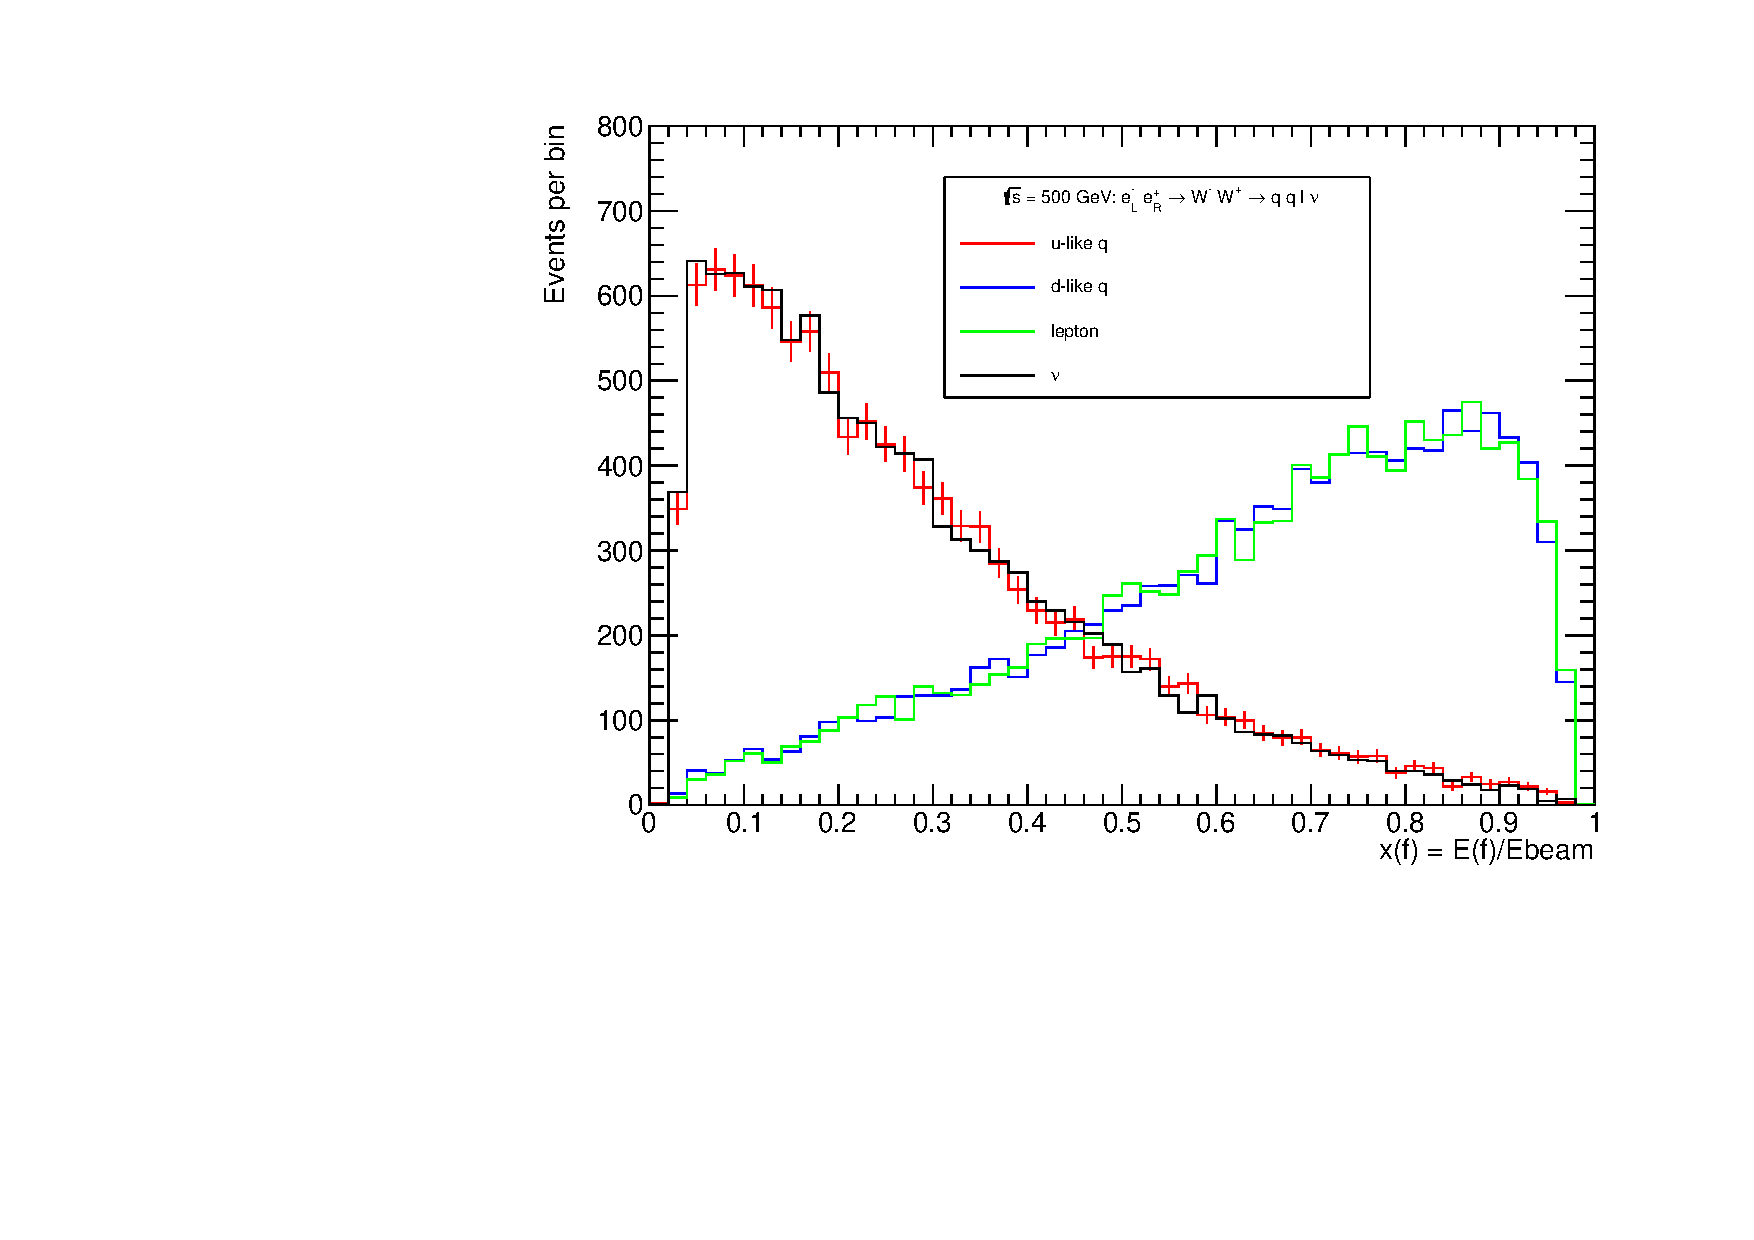
\includegraphics[width=0.48\textwidth]{hxLR.pdf}
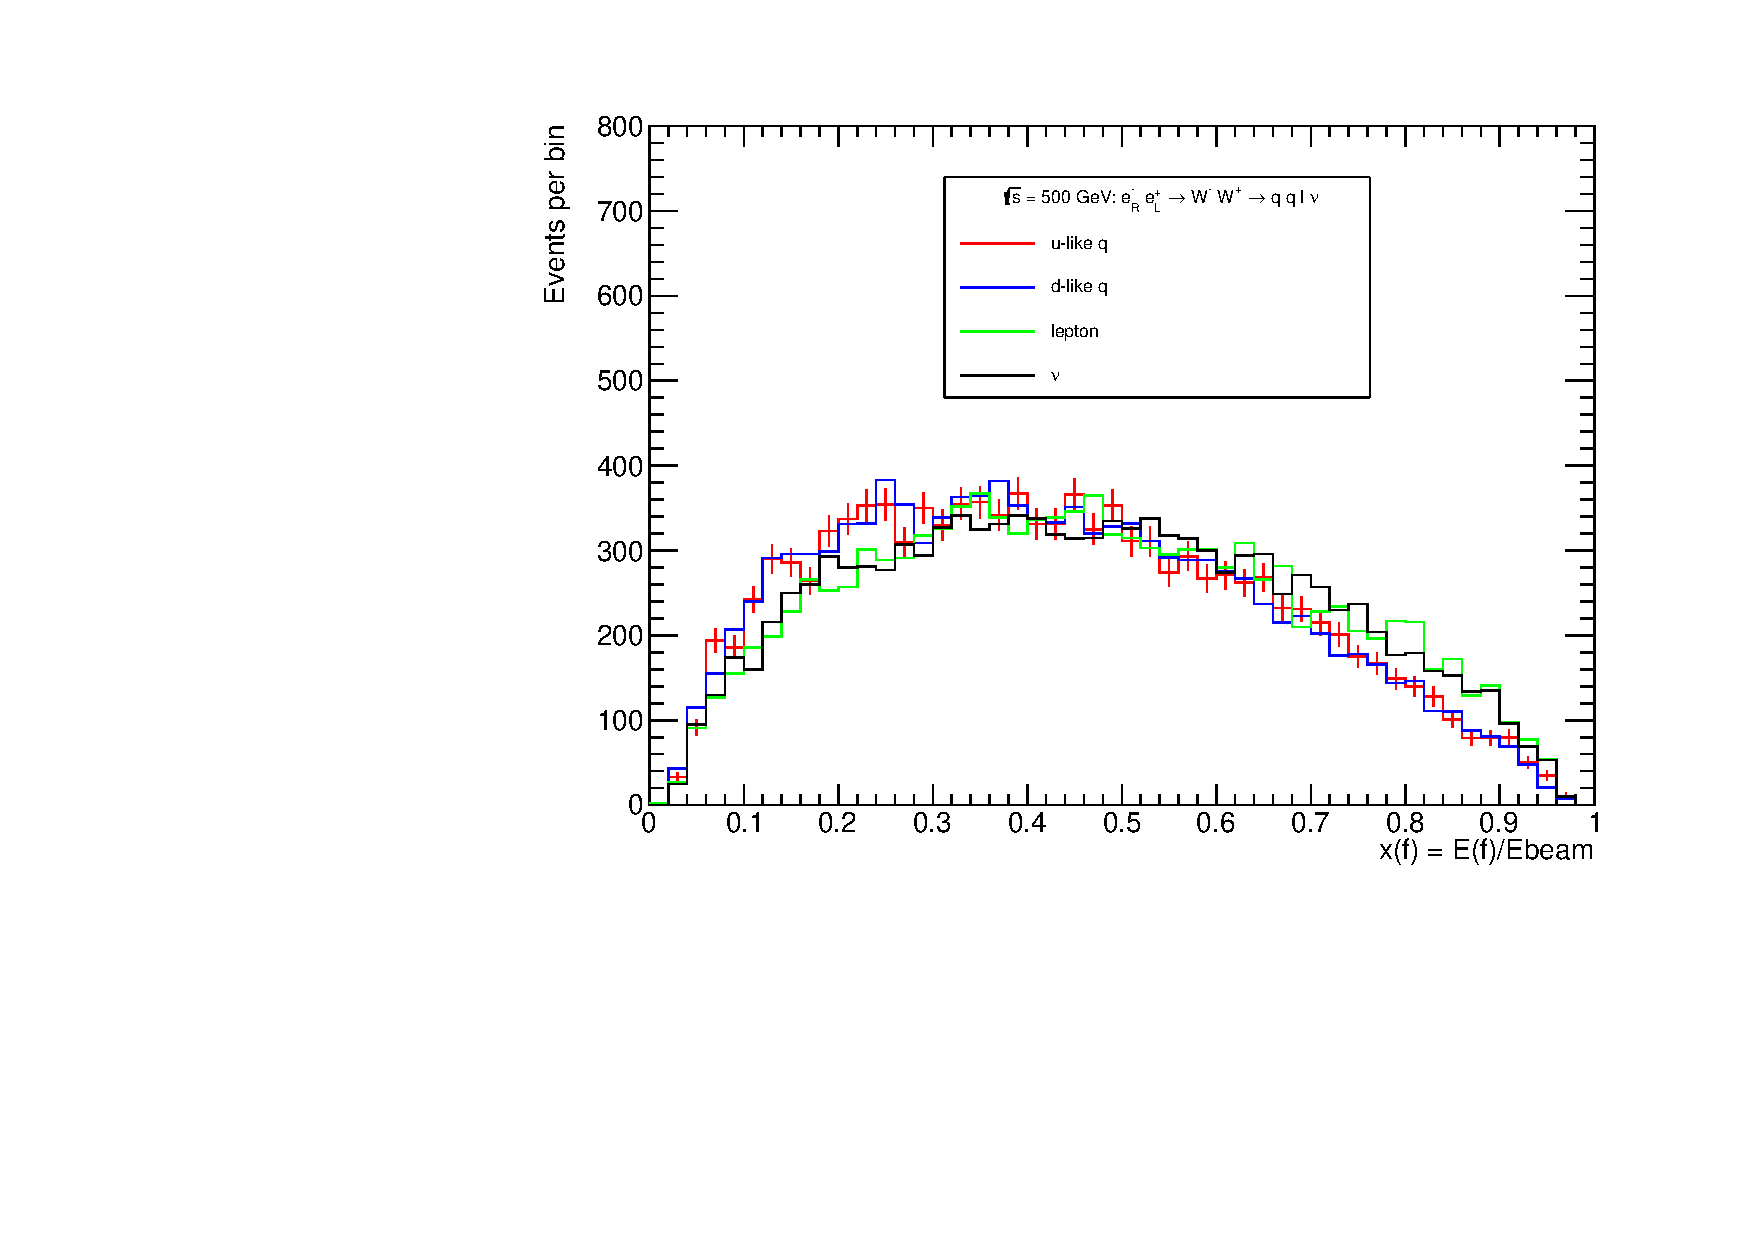
\includegraphics[width=0.48\textwidth]{hxRL.pdf}
\caption{The fractional energy partitioning of the true fermions with $\ell = \mu,\tau$, $100\%$ polarization for the initial state helicities LR(Left) and RL(Right) at center of mass energy 500 GeV. In the LR configuration the charged lepton and down-like quark take the majority of the beam energy. In RL the energy partitioning is even between the four fermions. }
\label{fig:Epartition}
\end{figure}

\begin{figure}


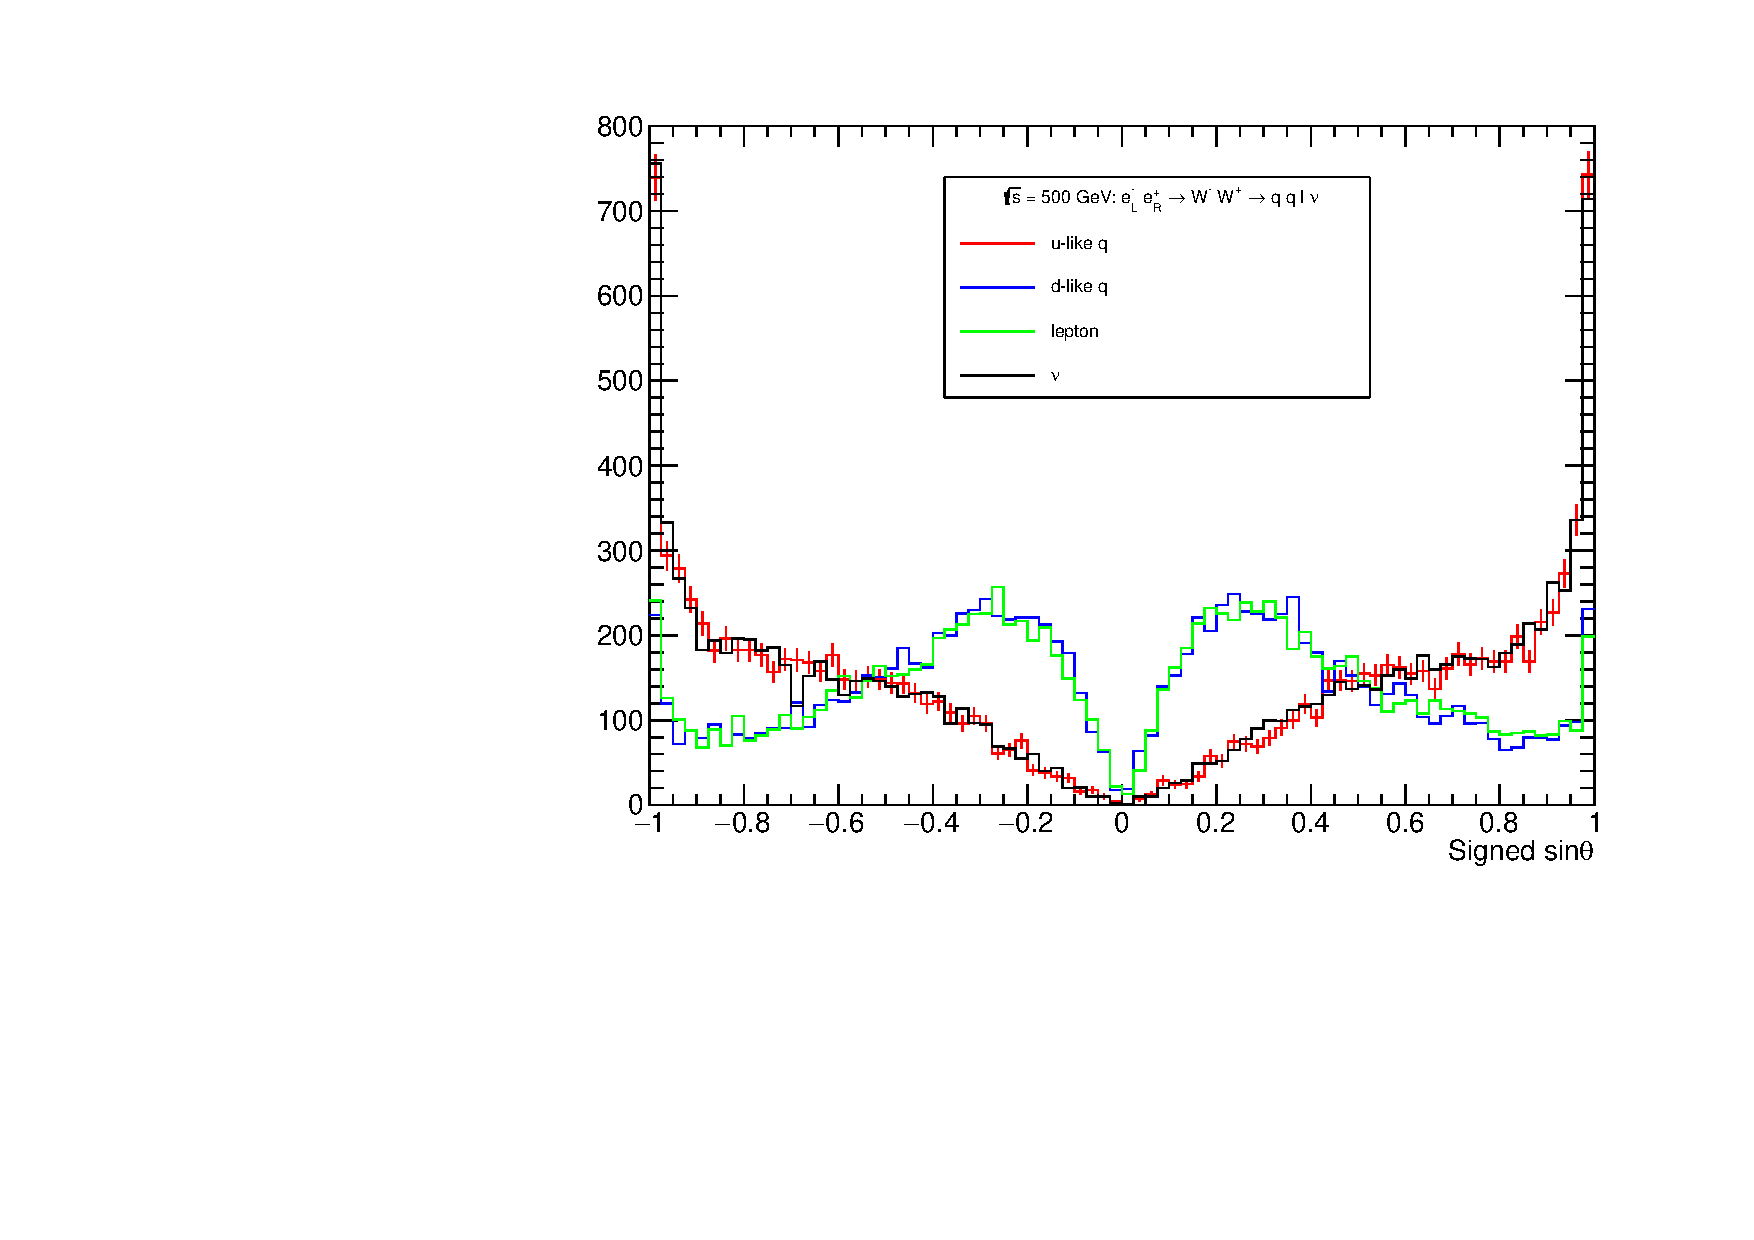
\includegraphics[width=0.48\textwidth]{hsLR.pdf}
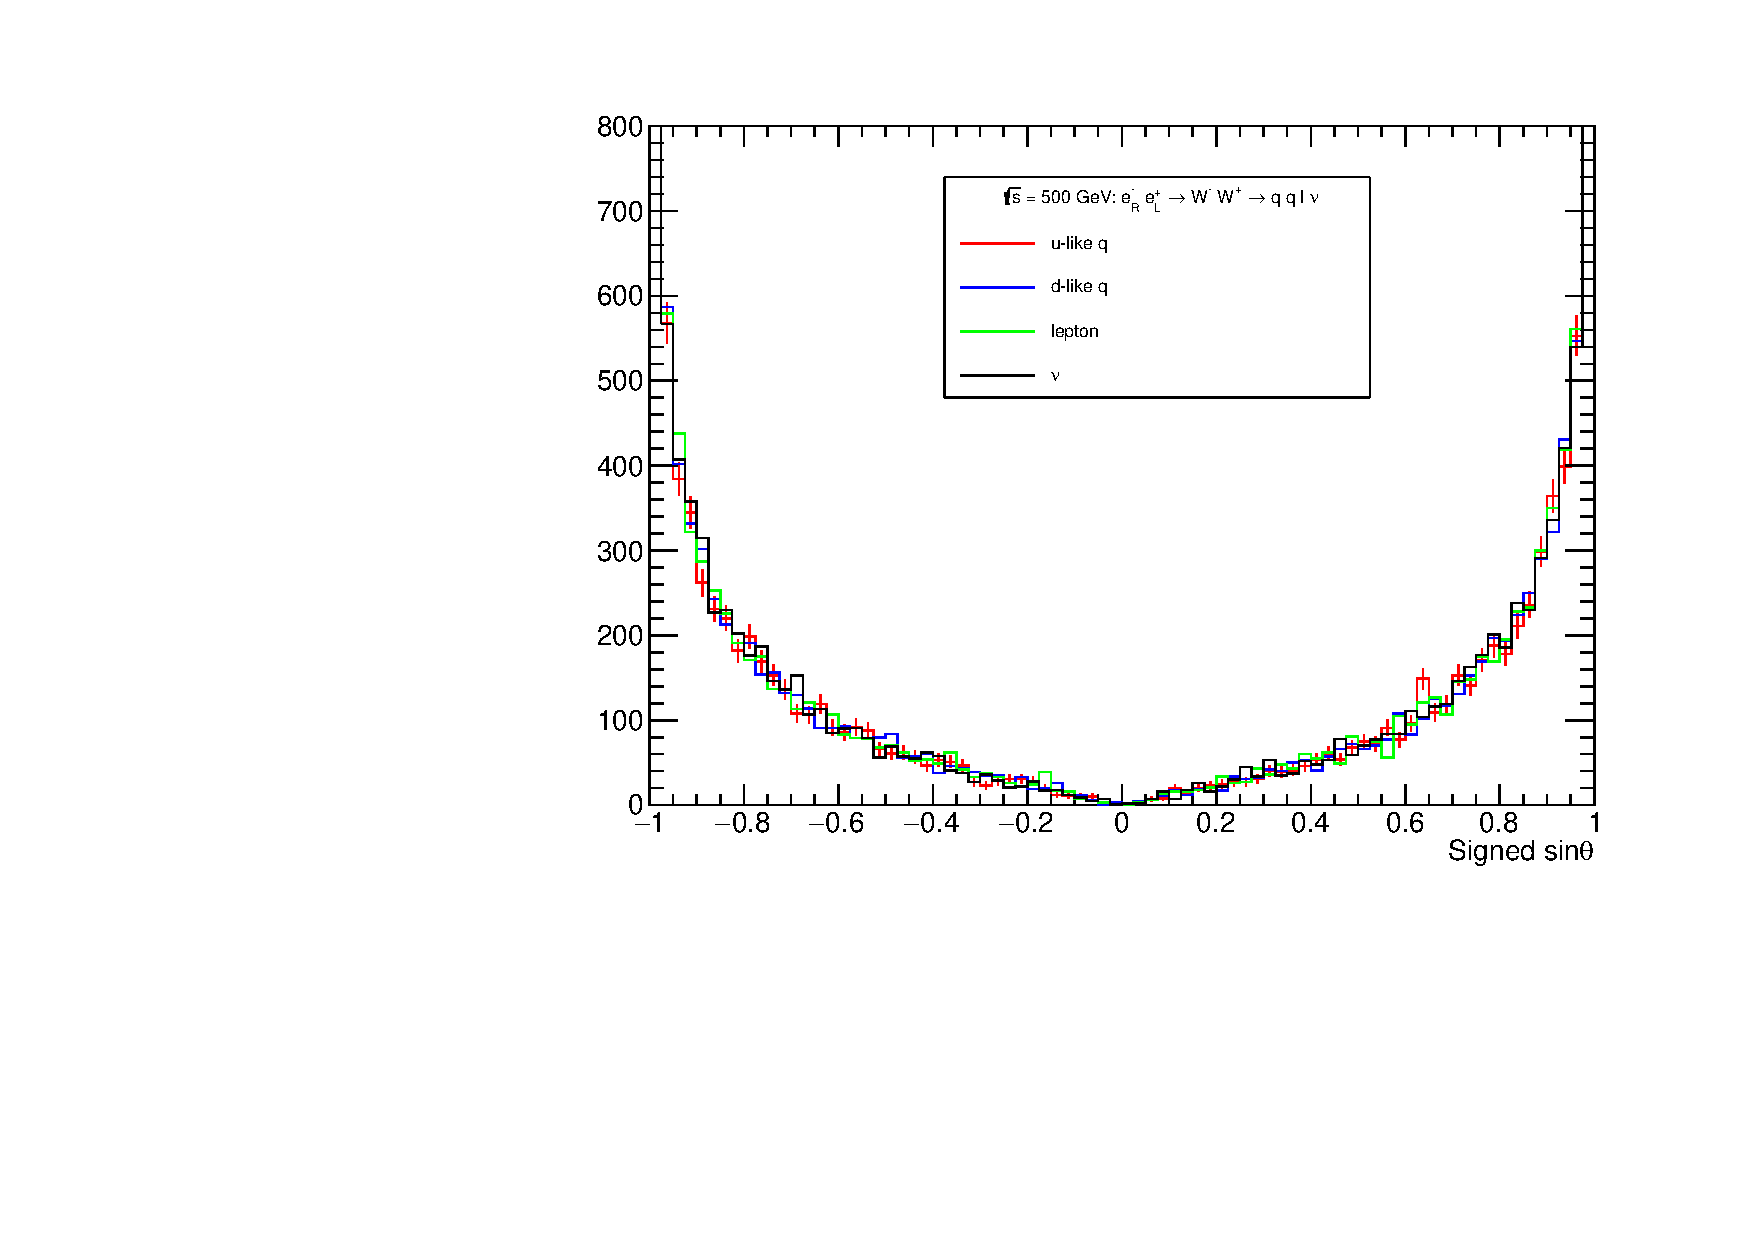
\includegraphics[width=0.48\textwidth]{hsRL.pdf}
\caption{The Signed sine of the polar angle of the true fermions with $\ell = \mu,\tau$. $100\%$ polarization for the initial state helicites. The sign of $sin\theta$ corresponds to the sign of $cos\theta$. As $sin\theta \rightarrow 0$ the fermion is forward in the detector but for $|sin\theta| \rightarrow 1$ the fermions become maximally transverse to the beam. In the LR configuration(Left) the charged lepton and down-like quark are scattered forward while the up-like quark and neutrino are ejected centrally into the detector. In the RL configuration(Right) all of the fermions are more centrally produced. }
\label{fig:fangles}
\end{figure}

After a lepton candidate has been selected, the remaining particles in the system are expected to form the hadronically decaying W-boson. However, the vector sum of the paricles  produces a distribution that is often in excess of the true hadonic mass. Variation between the true and measured mass naturally arise due to the mismeasurment of particles -- especially neutral hadrons, as well as particles lost beyond the acceptance range of the detector. Neither of these effects should create a systematic excess in the hadronic mass. The nature of the excess can be understood through the kinematics of the WW in the LR and RL configurations shown in Figure \ref{fig:Epartition} and \ref{fig:fangles}. The highest yielding configuration, LR, typically has two fermions that are forward in the detector which both typically have a large fraction of the beam energy. These fermions are susceptible to pile-up scattering into the detector and mixing directly into the reconstructed jets. To combat effects of pile-up, jet clustering algorithms via FastJet\cite{fastjet} are used.  The standard approach for pileup mitigation is to use the kT algorithm\cite{kt} and tune the R parameter such that the pile-up particles are associated with beam jets while the desired particles are not. With successful kT clustering the beam jets can be thrown away without damaging the reconstruction of the desired event. However, this approach only works well in events that are centrally produced.  The pile-up overlap in the forward topology with the kT algorithm  based clustering leads to rejecting desired particles and severe undermeasuremnt of the W mass. The solution to proper pileup mitigation is through the precise removal of foreign particles inside the reconstructed jets.  This can be achieved by using the standard JADE algorithm and mass based cut-off parameter $y_{cut} > y_{ij}$ where $y_{ij} = M_{ij}^2 / Q^2$ with $M_{ij}$ being the invariant mass of the pair of objects being combined and $Q^2$ being the visible energy in the $e^{+}e^{-}$ annihilation \cite{ycut}.  The mass of individually reconstructed jets can be controlled by tuning the $y_{cut}$ parameter. For large values, $y_{cut} =1\times10^{-3}$, a single massive jet is reconstructed. In the limit that $y_{cut}$ becomes infinitely small the number of jets reconstructed converges to the number of reconstructed particles.  The best $y_{cut}$ value is the value that forms mini-jets that safely couple together hard and soft emissions from  the original quark jet while segregating pile-up into its own mini-jets. The mini-jets are then subjected to kinematic cuts that maximize the pileup rejection and minimize the difference  between the true and measured hadronic W mass. 	The best combination of $y_{cut}$ and mini-jet kinematic cuts are found by examining the $100\%$ polarized LR signal muon dataset.  Two statisical estimators are used to maximize the pile-up rejection, both which come from the distribution of $M_{qq}^{meas} - M_{qq}^{true}$. This binned mass difference distribution is created from the subset of mini-jets that arise from clustering with a given $y_{cut}$ and also pass some jet veto cuts $p_{Tjet} > x$ and $|cos\theta_{jet}| < y$. The estimators, from the distribution, are the Full Width Half Maximum(FWHM) and the number of entries in the Mode.  
Using estimators calculated from a binned histogram creates unwanted sensitivity to bin size. To reduce sensitivity to binning, the mode is defined as the bin with the most entries. The ``mode entries" is the number of entries in the mode bin plus the number of entries in the mode bins nearest neighbors. For the FWHM, the mass distribution is assumed to be monotonically decreasing around the half maxmimum. To create a more sensitive continuous distribution of the FWHM,  the FWHM is weighted towards the bin center of the two bins around (above/below) the half maximum. The results of the optimization are shown in Figure \ref{fig:supmass} and various $y_{cut}$'s are shown in comparison to the optimal configuration in Figure \ref{fig:supdiff}. The leading result uses $y_{cut} = 5\times 10^{-5}$, mini jet $P_T > 2$ GeV, and has no $|\cos \theta|$ requirement. 

\begin{figure}
    \centering
    \begin{minipage}{0.49\textwidth}
        \centering
        
        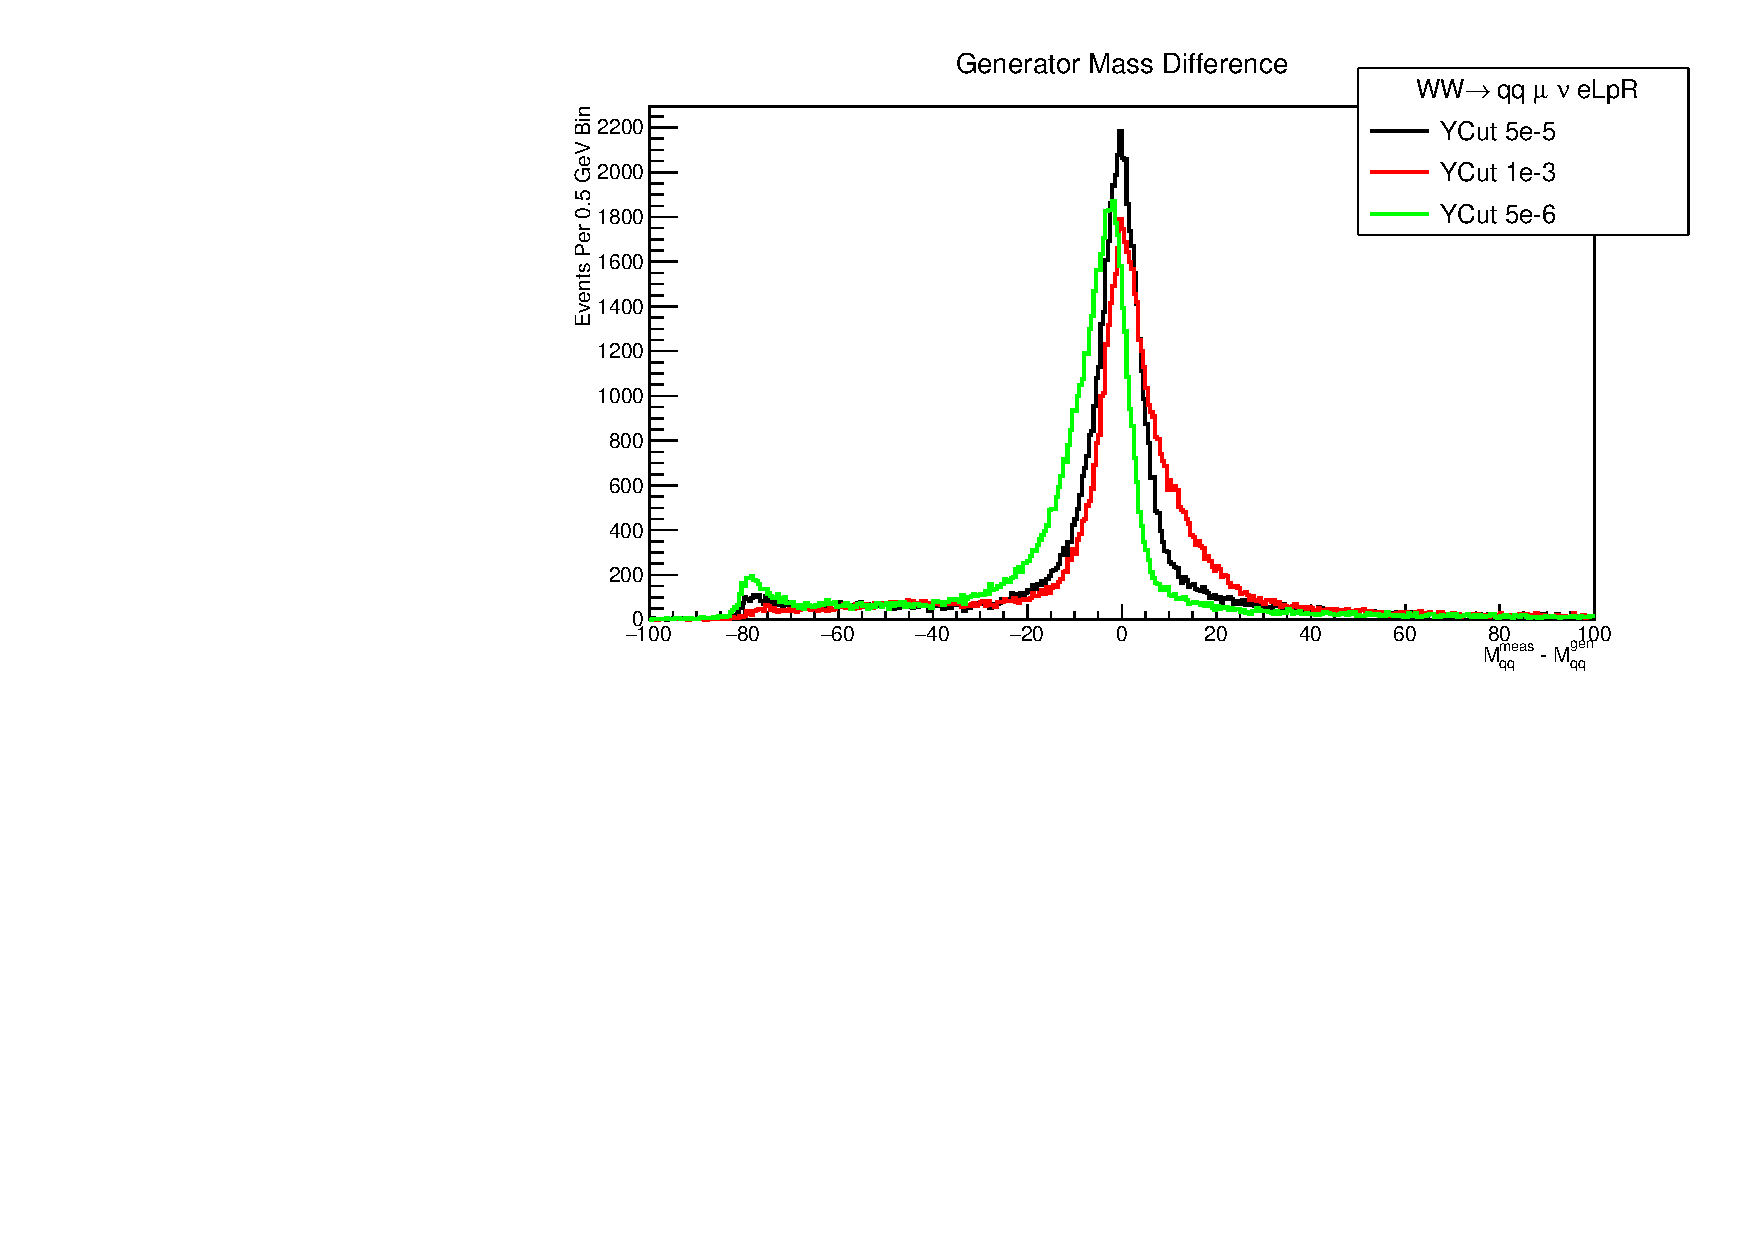
\includegraphics[width=0.99\textwidth]{SupDiff.pdf} % first figure itself
        \caption{Comparison of mass difference distributions with different $y_{cut}$ values and the same mini-jet cut $P_T > 2$. $y_{cut} = 1\times 10^{-3}$ results in massive jets that are not separated from pile-up and insensitive to small kinematic cuts. $y_{cut} = 5\times 10^{-5}$ has the best balance between jet clustering and mini-jet cuts. $y_{cut} = 5\times 10^{-6}$ yields a highly fragmented version of the jets where the mini-jets are not distinguishable from pile-up and are thrown out, resulting in the small peak around -80 GeV where the hadronic W is completely thrown out.  }
        \label{fig:supdiff}
    \end{minipage}\hfill
    \begin{minipage}{0.49\textwidth}
        \centering
        
        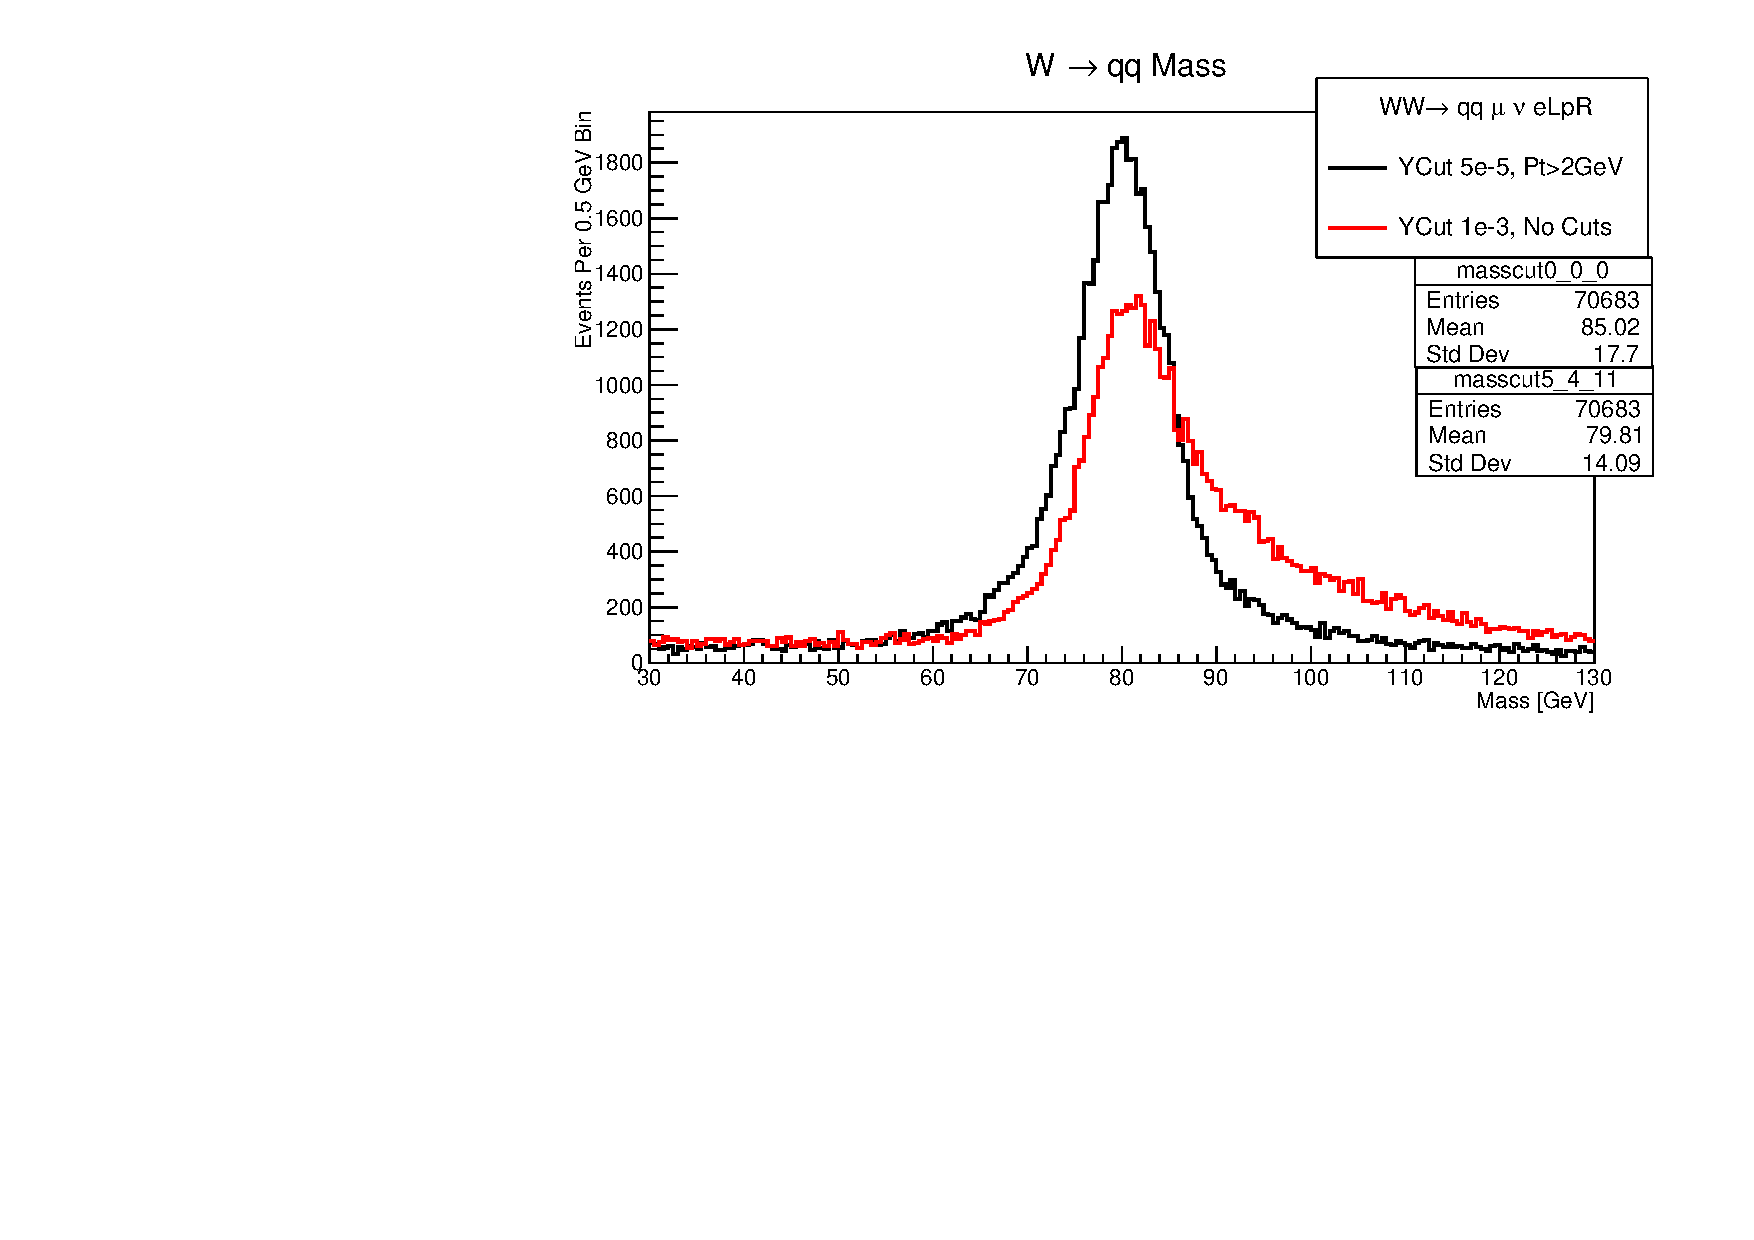
\includegraphics[width=0.99\textwidth]{SupMass.pdf} % second figure itself
        \caption{The increase of quality of the hadronic mass is shown between the red curve which is the raw hadronic system after lepton identification versus the black curve which is subjected to the pile-up mitigation with $y_{cut} = 5\times10^{-5}$ and mini jet $P_T > 2$ GeV. On average the excess in mass is reduced by $\approx 5$ GeV. }
        \label{fig:supmass}
    \end{minipage}
\end{figure}


\subsection{EventSelection}
\label{subsec:EventSelection}
The W-pair selection has been optimized for a Monte Carlo sample of 1600 $\text{fb}^{−1}$ with the $(-0.8,+0.3)$ beam scenario and is based on the selection in \cite{ivan}. The selection includes the full 2,4,6 fermion and Higgs SM background, and is performed with two independent subsets, a tight and loose selection. The tight selection uses the prompt muon cone to identify signal events that contain both prompt and non-prompt muons and electrons. The tight selection is inefficient in collecting hadronic taus, so, the loose selection, using the inclusive tau cone, is designed to recover the efficiency of hadronic taus and other problematic events. The selection criteria is as follows:
\begin{itemize}
\item N Leptons $\geq 1$
\item Track Multiplicity $> 10$  
\item Visible Pt $> 5$ GeV  
\item $E_{vis} < 500$ GeV 
\item $E_{com} > 100$ GeV
\item $40<M_{qq}<120$ GeV
\item  $-qcos\theta_W < -0.95$
\item  $m^2_{\nu recoil} < 135,000 \, \, \text{GeV}^2$
\end{itemize}

The track multiplicity and $E_{com}$ target 2 fermion backgrounds. $E_{com}$ is the rest-frame energy that consists of the visible and inferred missing energy. The missing energy is treated as a single neutrino with zero mass such that $E_{com} = E_{vis} + |P_{miss}| \, \,  \, \text{and} \, \, P^\mu_{miss} = (|P_{miss}| , -\sum{\vec{p}_{vis}})$. The Visible $P_T$ is scalar sum of all measured transverse momentum and $E_{vis}$ is the sum of all reconstructed visible energy in an event. The $P_T$ and $E_{vis}$ cuts target processes that do not have a genuine missing energy from a neutrino. The hadronic W-mass $M_{qq}$ requirement forces the hadronic system to be ``W-like" and the recoil mass, $m_{\nu recoil}$, uniquely requires the visible system to be recoiling against an invisible system with little to no mass. The recoil mass is defined as $m^2_{\nu recoil} = s + M^2_{vis} - 2\sqrt{s}E_{vis} \, \, \text{and} \, \, M^2_{vis} = ( P^{\mu}_{qq} +  P^{\mu}_{\ell})^2$. The W-scattering cut $-q\cos\theta_W$ is the angle of deflection of the system identified as $W^-$ with respect to the $e^-$ beam axis and is implemented to limit backward scattering.  The charge of the lepton is extracted from the leading momentum track from candidates with 1, 2, or 4 tracks, or in the case of 3 tracks, the charge is the sum of the three track charges. The hadronic system is then tagged with the opposite charge.  This procedure results in the correct charge assignment of the lepton before selection cuts for about $98.9\%$ of prompt muons, $94.8\%$ of prompt electrons, and $95.9\%$ of taus. Following the event selection the correct charge assignment increases to $99.9\%$ for prompt muons, $98.3\%$ for prompt electrons, and $98.8\%$ for taus. The selection variables for signal and background are shown after the lepton requirement in Figure \ref{fig:stacks1} in the Appendix.  The details of the tight and loose selection for (-0.8,+0.3) at 1600$\text{fb}^{-1}$ are summarized in Table \ref{tab:selection}. The selections in Table \ref{tab:selection} differ by the veto of the tight lepton in the loose selection, where the preference for any event is to always choose a tight lepton over loose. The primary selection also includes only ``WW-like" signal, this type of signal is such that both of the true fermion pairs invariant masses are each within $\pm10$ GeV of the nominal W mass. If an event contains a fermion pair that is outside the WW-like range, it is designated as an off-shell(O.S) event and is placed in a different category. The selection cuts are optimized to maximize the efficiency and purity of the total signal for the tight selection. The results are summarized with the two selection cones with and without O.S. events in Table \ref{tab:summary}. The final results for the mass inclusive selection yields a signal efficiency of $58\%$ with only a $9\%$ of background contaminating selected events. The W-boson invariant mass after selection is shown with mass resolution in Figure \ref{fig:money}


\begin{table}

\caption{The tight and loose selection for 1600 $\text{fb}^{-1}$ (-0.8,+0.3). The tight selection is most efficient with prompt leptons with $69\%$ and $65\%$  for muons and electrons respectively, but struggles to efficiently reconstruct taus. The loose selection recovers $10\%$ of the tau efficiency and is inefficient for prompt leptons because of the tight lepton veto. The tight lepton veto enforces the orthogonality of the selections gives preference toward better lepton candidates. The signal categories Base Evts. only include events in which the true W mass of both fermion pairs are within 10 GeV of the nominal W mass.}
\label{tab:selection}
 \scriptsize
 Tight selection with muon cone
   \begin{tabular}{|p{0.11\textwidth}|p{0.11\textwidth}p{0.11\textwidth}p{0.11\textwidth}p{0.11\textwidth}p{0.11\textwidth}p{0.11\textwidth}p{0.11\textwidth}p{0.1\textwidth}|}
\hline 
   & Prompt $\mu$ & Prompt $e$ & $\tau$ & Tot. Sig. & 2f & 4f & 6f & Higgs \\ \hline 
Base Evts &\num{3.87e+06 } & \num{3.89e+06 } & \num{3.90e+06} &\num{1.17e+07} & \num{4.22e+07} & \num{3.22e+07} & \num{2.14e+05} & \num{4.12e+05} \\ 

Lepton &\num{3.31e+06 } & \num{3.20e+06 } & \num{2.28e+06} &\num{8.78e+06} & \num{1.15e+07} & \num{1.18e+07} & \num{1.63e+05} & \num{1.15e+05} \\ 
 
$E_{vis}$ &\num{3.28e+06 } & \num{3.11e+06 } & \num{2.27e+06} &\num{8.67e+06} & \num{1.06e+07} & \num{1.15e+07} & \num{1.62e+05} & \num{1.11e+05} \\ 
 
N Tracks &\num{3.19e+06 } & \num{3.03e+06 } & \num{2.21e+06} &\num{8.43e+06} & \num{2.54e+06} & \num{2.59e+06} & \num{1.49e+05} & \num{8.89e+04} \\ 
 
$-qcos\theta$ &\num{3.18e+06 } & \num{3.01e+06 } & \num{2.18e+06} &\num{8.37e+06} & \num{2.19e+06} & \num{2.26e+06} & \num{1.44e+05} & \num{8.52e+04} \\ 
 
$M_{qq}$ $>$40 &\num{2.94e+06 } & \num{2.80e+06 } & \num{2.03e+06} &\num{7.77e+06} & \num{1.13e+06} & \num{1.33e+06} & \num{1.42e+05} & \num{7.56e+04} \\ 
 
$M_{qq}$ $<$120 &\num{2.72e+06 } & \num{2.57e+06 } & \num{1.83e+06} &\num{7.13e+06} & \num{5.68e+05} & \num{2.68e+05} & \num{2.02e+04} & \num{2.97e+04} \\ 
 
$E_{com}$ &\num{2.72e+06 } & \num{2.57e+06 } & \num{1.83e+06} &\num{7.13e+06} & \num{5.58e+05} & \num{2.65e+05} & \num{2.02e+04} & \num{2.96e+04} \\ 

Pt vis. &\num{2.69e+06 } & \num{2.55e+06 } & \num{1.81e+06} &\num{7.05e+06} & \num{3.21e+05} & \num{2.37e+05} & \num{2.01e+04} & \num{2.94e+04} \\ 

$m^2_{\nu recoil}$ &\num{2.69e+06 } & \num{2.54e+06 } & \num{1.80e+06} &\num{7.03e+06} & \num{2.93e+05} & \num{2.02e+05} & \num{1.94e+04} & \num{2.23e+04} \\ 
\hline 

 $\epsilon$ & $0.694 $ & $0.654 $ & $0.462$ &  $0.603 $ & $0.0069 $ & $0.00626 $ & $0.0905 $ & $0.0541 $ \\ 
 
 			& $\pm$0.002 & $\pm$0.002 & $\pm$0.003 & $\pm$0.002 & $\pm$ 0.0001 & $\pm$\num{8e-05} & $\pm$ 0.0002 & $\pm$0.0005 \\
\hline
\end{tabular}
\quad \quad \\
Loose selection with tau cone\\
\begin{tabular}{|p{0.11\textwidth}|p{0.11\textwidth}p{0.11\textwidth}p{0.11\textwidth}p{0.11\textwidth}p{0.11\textwidth}p{0.11\textwidth}p{0.11\textwidth}p{0.1\textwidth}|}
\hline 
   & Prompt $\mu$ & Prompt $e$ & $\tau$ & Tot. Sig. & 2f & 4f & 6f & Higgs \\ \hline 
Base Evts &\num{3.87e+06 } & \num{3.89e+06 } & \num{3.90e+06} &\num{1.17e+07} & \num{4.22e+07} & \num{3.22e+07} & \num{2.14e+05} & \num{4.12e+05} \\ 
 
Lepton &\num{3.36e+06 } & \num{3.30e+06 } & \num{2.82e+06} &\num{9.48e+06} & \num{1.30e+07} & \num{1.36e+07} & \num{1.77e+05} & \num{1.38e+05} \\ 

Tight Veto &\num{7.72e+04 } & \num{1.28e+05 } & \num{5.70e+05} &\num{7.76e+05} & \num{1.93e+06} & \num{2.15e+06} & \num{1.61e+04} & \num{3.12e+04} \\ 
 
$E_{vis}$ &\num{7.64e+04 } & \num{1.26e+05 } & \num{5.70e+05} &\num{7.72e+05} & \num{1.82e+06} & \num{1.94e+06} & \num{1.54e+04} & \num{3.02e+04} \\ 

N Tracks &\num{7.37e+04 } & \num{1.21e+05 } & \num{5.54e+05} &\num{7.49e+05} & \num{1.50e+06} & \num{1.64e+06} & \num{1.51e+04} & \num{2.71e+04} \\ 
 
$-qcos\theta$ &\num{6.30e+04 } & \num{1.12e+05 } & \num{5.32e+05} &\num{7.07e+05} & \num{1.11e+06} & \num{1.41e+06} & \num{1.45e+04} & \num{2.56e+04} \\ 
 
$M_{qq}$ $>$ 40 &\num{4.92e+04 } & \num{9.72e+04 } & \num{4.86e+05} &\num{6.33e+05} & \num{5.98e+05} & \num{1.30e+06} & \num{1.44e+04} & \num{2.33e+04} \\ 

$M_{qq}$ $<$ 120 &\num{4.04e+04 } & \num{7.81e+04 } & \num{4.16e+05} &\num{5.35e+05} & \num{2.58e+05} & \num{1.11e+05} & \num{1.11e+03} & \num{1.24e+04} \\ 
 
$E_{com}$ &\num{4.04e+04 } & \num{7.81e+04 } & \num{4.16e+05} &\num{5.34e+05} & \num{2.50e+05} & \num{1.10e+05} & \num{1.11e+03} & \num{1.24e+04} \\ 

Pt vis. &\num{4.00e+04 } & \num{7.74e+04 } & \num{4.12e+05} &\num{5.29e+05} & \num{1.17e+05} & \num{1.01e+05} & \num{1.11e+03} & \num{1.23e+04} \\ 
 
$m^2_{\nu recoil}$ &\num{3.94e+04 } & \num{7.70e+04 } & \num{4.07e+05} &\num{5.24e+05} & \num{1.02e+05} & \num{7.59e+04} & \num{1.02e+03} & \num{9.73e+03} \\ 
\hline 
 $\epsilon$ & $0.0102 $ & $0.0198 $ & $0.105 $ &  $0.0449 $ & $0.00241 $ & $0.00236 $ & $0.00474 $ & $0.0236 $ \\ 

  	     & $\pm 0.005$ & $\pm 0.0007$ & $\pm 0.002$ & $\pm 0.0007$ & $\pm$\num{3e-05} & $\pm$\num{4e-05} & $\pm$\num{7e-05} & $\pm$0.0002 \\

 \hline
 \end{tabular}

\end{table}



\begin{table}
\caption{Selection summary showing the number of background events that pass the event selection, efficiency, and purity for the tight selection or combined selections and with or without the off-shell contributions.  The O.S. contributions are less efficiently reconstructed so their inclusion reduces the overall signal efficiency but boosts the purity by increasing the base number of signal events that can be selected. Selection is performed with 1600 $\text{fb}^{-1}$ in (-0.8, +0.3). }
\label{tab:summary}
 \begin{tabular}{ |p{0.12\textwidth}|p{0.12\textwidth}p{0.15\textwidth}|p{0.12\textwidth}|p{0.12\textwidth}p{0.15\textwidth}p{0.12\textwidth}|} 
 \hline 
   &  \multicolumn{3}{|l|}{Tight Selection} &  \multicolumn{3}{|l|}{ Tight + Loose Sel.}  \\  \hline  
 & Sel. Total & Efficiency & Purity & Sel. Total & Efficiency & Purity \\ 
 \hline  
 Bkg. & \num{5.36e+05} & & & \num{7.25e+05} & &  \\ 
 Signal & \num{4.49e+06} & 0.578 $\pm$ 0.002 & 0.893  & \num{4.93e+06} & 0.635 $\pm$ 0.002 & 0.872 \\ 
 Sig.+O.S. & \num{6.93e+06} & 0.541 $\pm$ 0.001 & 0.928 & \num{7.47e+06} & 0.584 $\pm$ 0.001 & 0.912 \\ 
\hline 
\end{tabular} 
\end{table}

\begin{figure}

\centering
    \begin{minipage}{0.49\textwidth}
        \centering
        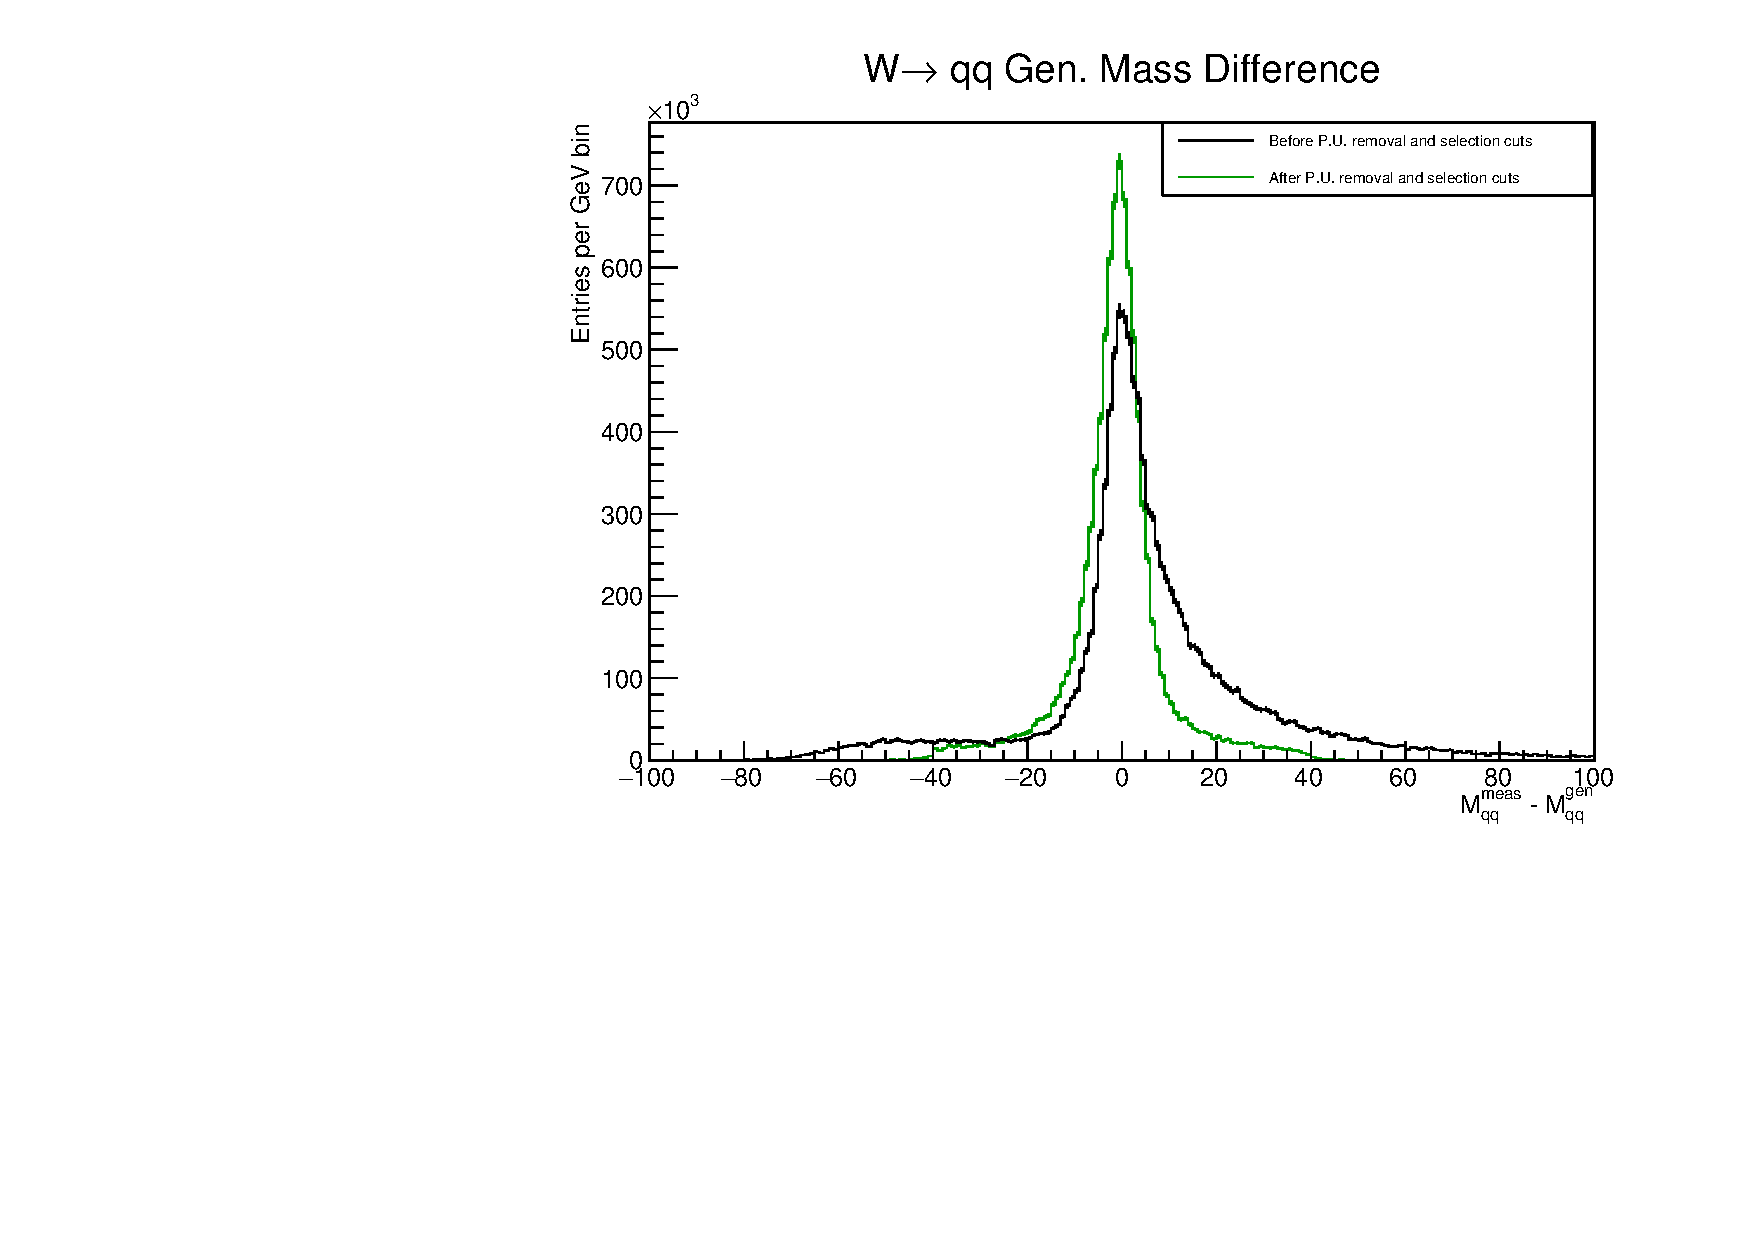
\includegraphics[width=0.99\textwidth]{moneymassdiff.pdf} % first figure itself
   
    \end{minipage}\hfill
    \begin{minipage}{0.49\textwidth}
        \centering
        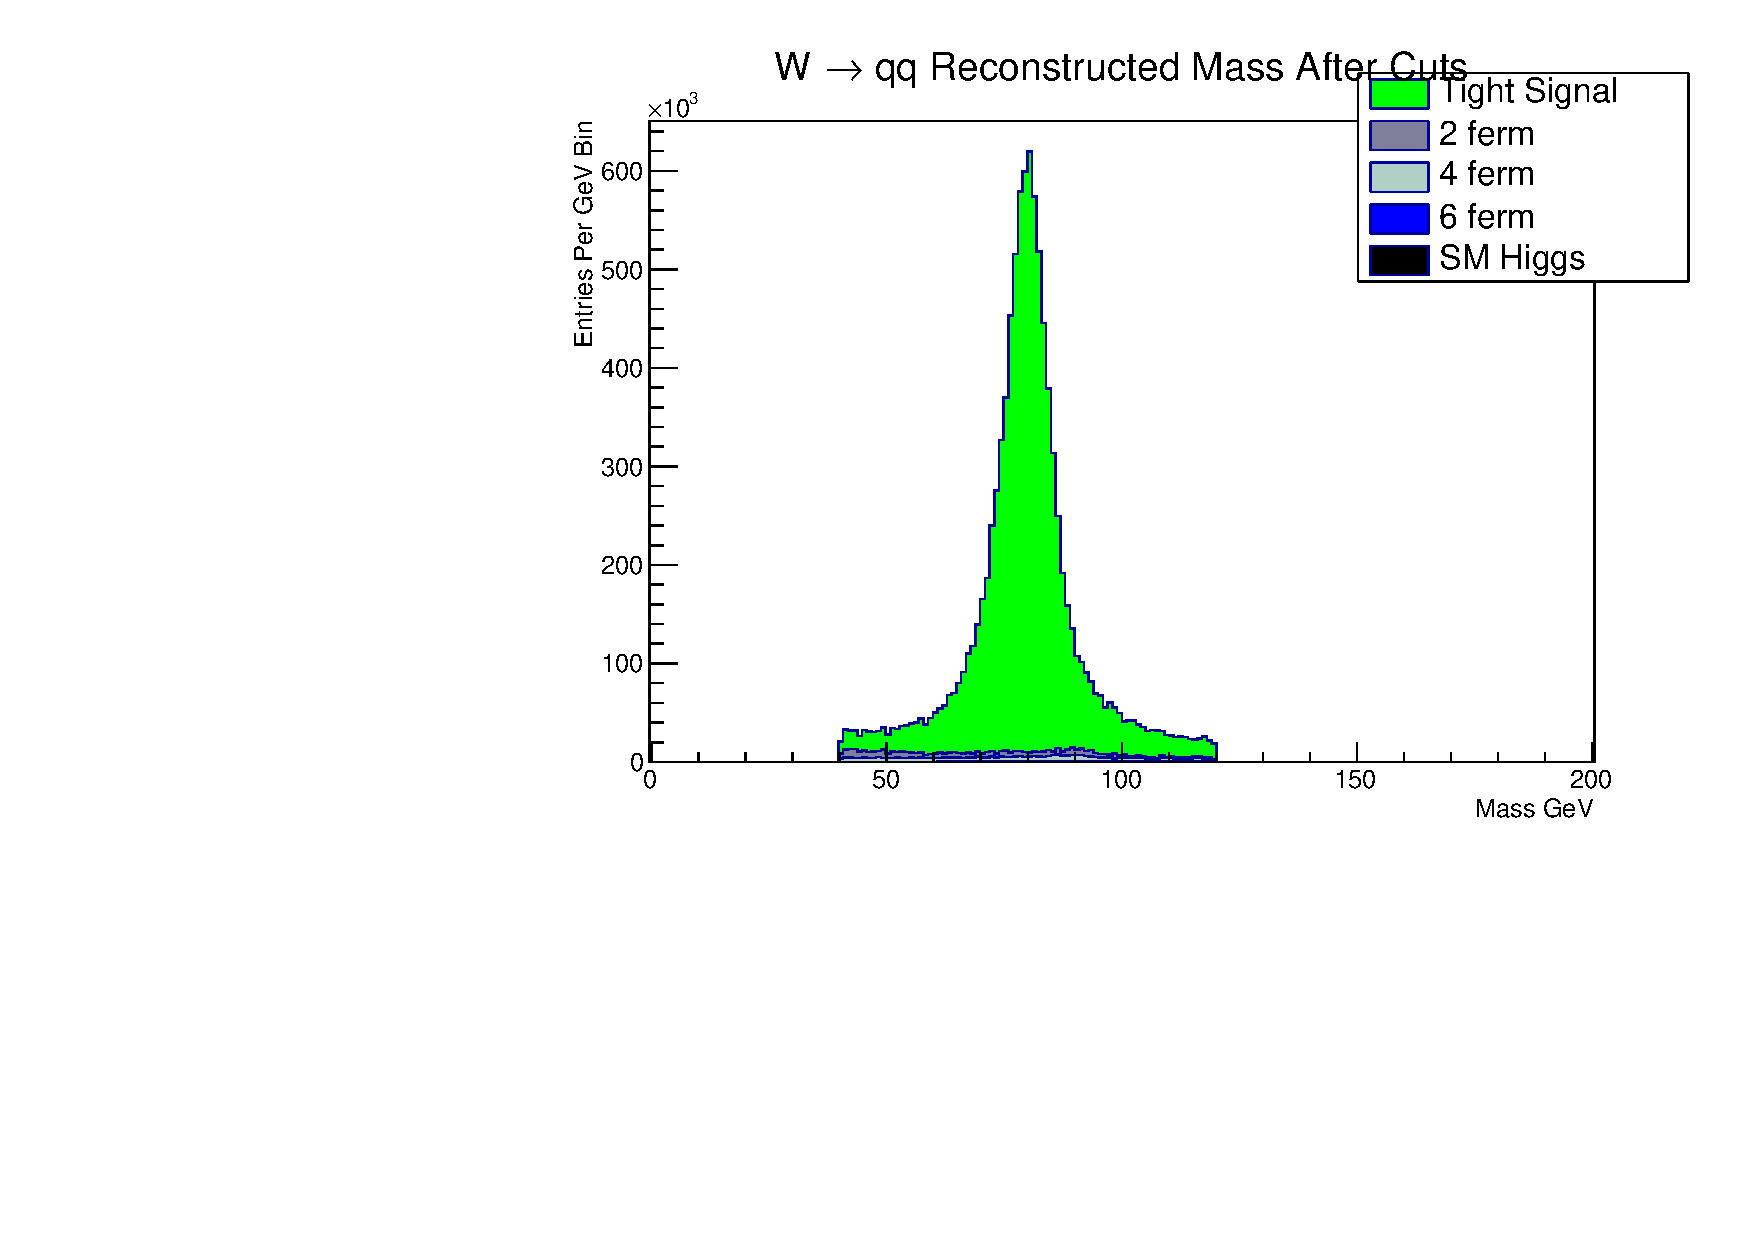
\includegraphics[width=0.99\textwidth]{mwhadCutsHist.pdf} % second figure itself
     
     \end{minipage}\\
     \caption{The right distribution is the mass of the hadronic W-boson after pile up removal and selection cuts against the remaining background events . The left distribution shows the resolution of the hadronic W mass with respect to the true mass in Monte Carlo before pile up removal and selection cuts and after pile up removal and selection cuts. The resolution shows a significant improvement in symmetry and events with excess mass are shifted centrally.  Uses 1600 $\text{fb}^{-1}$ in (-0.8,+0.3). 
}
\label{fig:money}
\end{figure}

\subsection{Results}
\label{subsec:wmass}

A Voigtian fit of the hadronic W mass is performed on the tight signal sample with the combined lepton categories shown in Figure \ref{fig:badfit}. The resulting fit models the shape and the mean of the distribution well but deviates around 90 GeV and edges of the fit window. The width of the fit is also in excess of the true width, which is about 2 GeV. This means the Voitigian model is indadequate in describing  the data, but, because shape is similar to data, the fitted model is used to understand the achievable mass resolution given a perfect model. Statistics consistent with 1600 $\text{fb}^{-1}$ (9.36M Events) are produced according the previously fitted model with a mean  $M_W = 79.7074$, width $\Gamma_W = 10.6972$ and $\sigma_W = 4.847 \times 10^{-7}$ and refitted to achieve the statistical error on the mean $\Delta M_W \text{(stat.)} = 2.4$ MeV with goodness-of-fit $\chi^2 / ndof = 67.8/77$. The toy model refit is also included in Figure \ref{fig:badfit}.
The cross-section and errors are extracted from Table \ref{tab:selection} according to the formula:
\begin{equation}
\sigma = \frac{N_S - N_B}{L \epsilon}
\end{equation}
where $N_S$ is the observed number of events that passes selection and $N_B$ is expected number of background events that contaminate the signal selection. The resulting statistical error on the cross-section with $\epsilon$, $L$, and $N_B$ known perfectly is $\frac{\Delta \sigma}{\sigma} = 0.04 \%$. Combining the errors for efficiency, poisson errors for $N_S$, and having  no background contribution, the resulting cross-section obtained in the combined selection is $7994 \pm 14 \, \, \text{fb}$
\begin{figure}

\centering
    \begin{minipage}{0.49\textwidth}
        \centering
        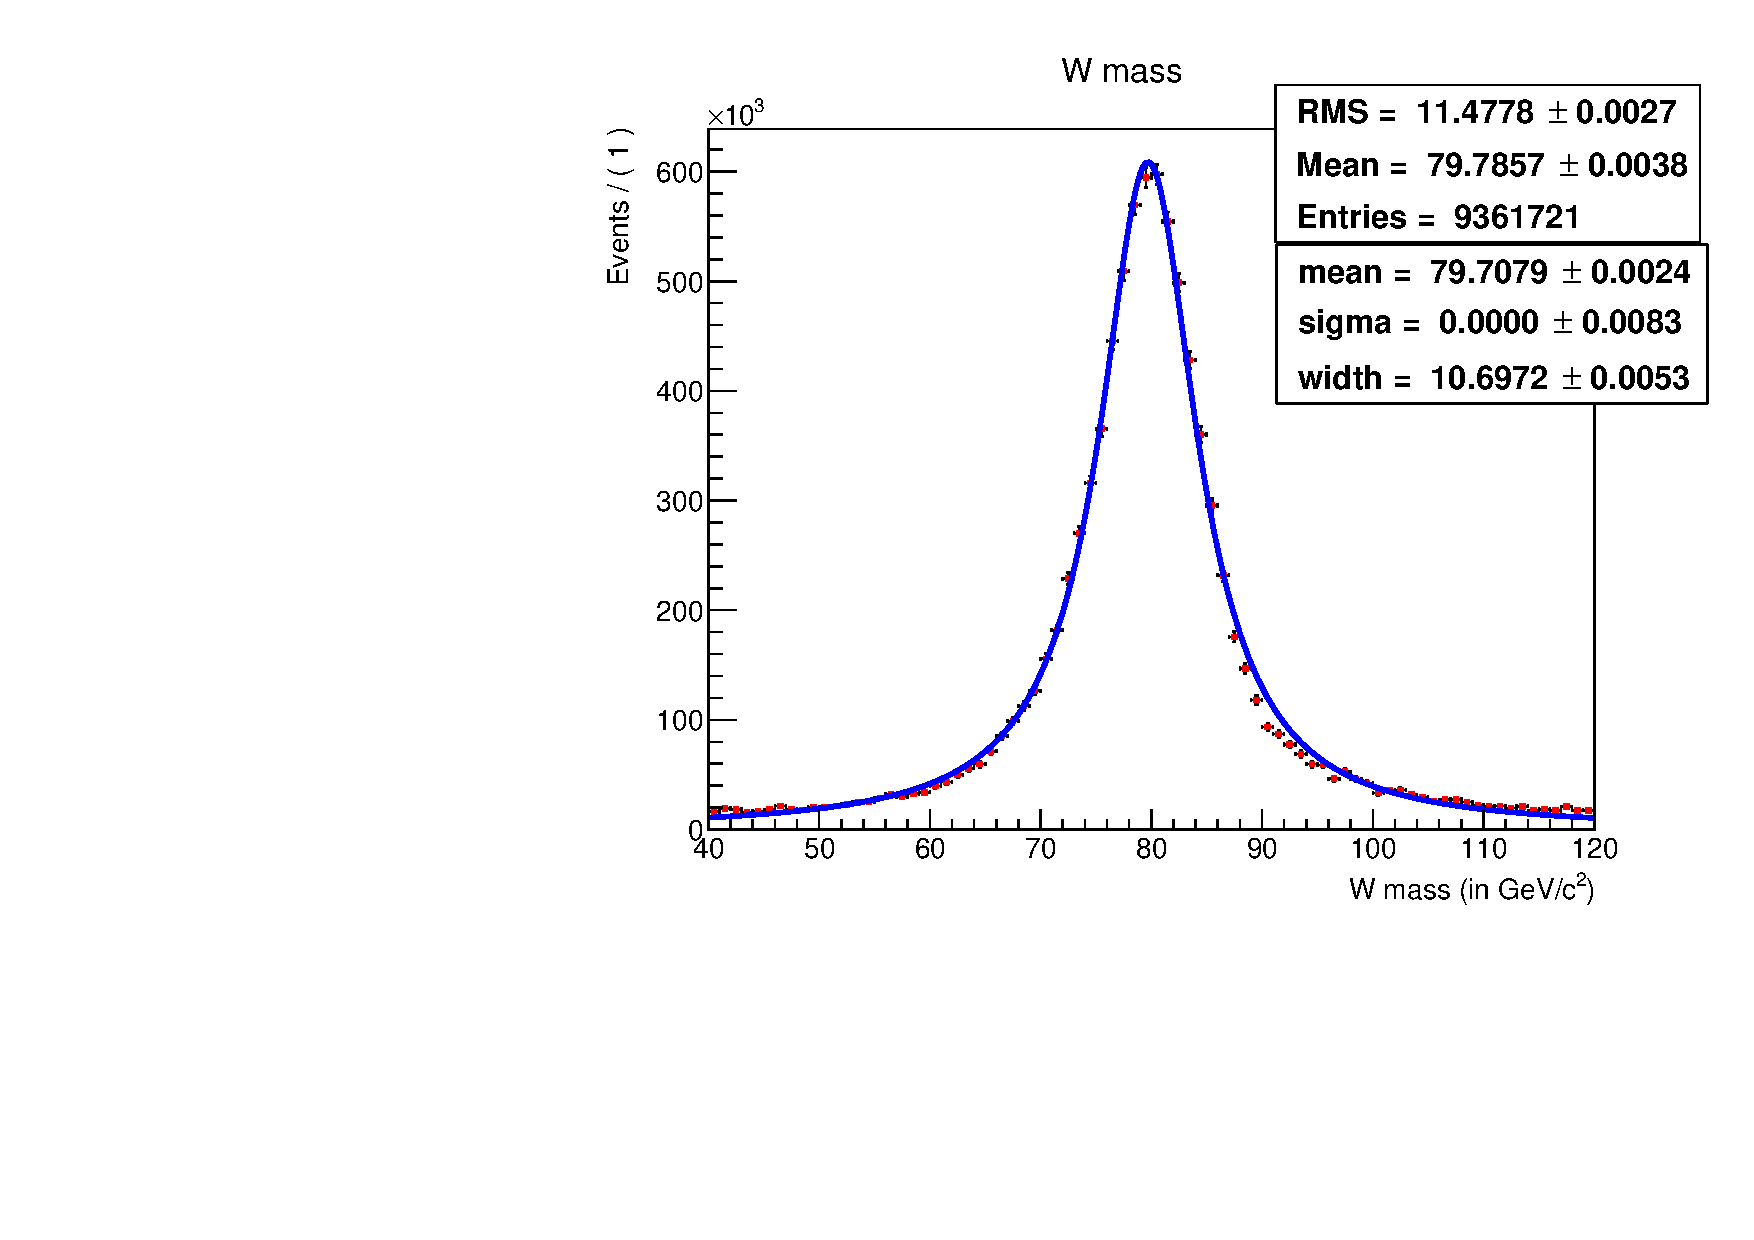
\includegraphics[width=0.99\textwidth]{WWSfit.pdf} % first figure itself
   
    \end{minipage}\hfill
    \begin{minipage}{0.49\textwidth}
        \centering
        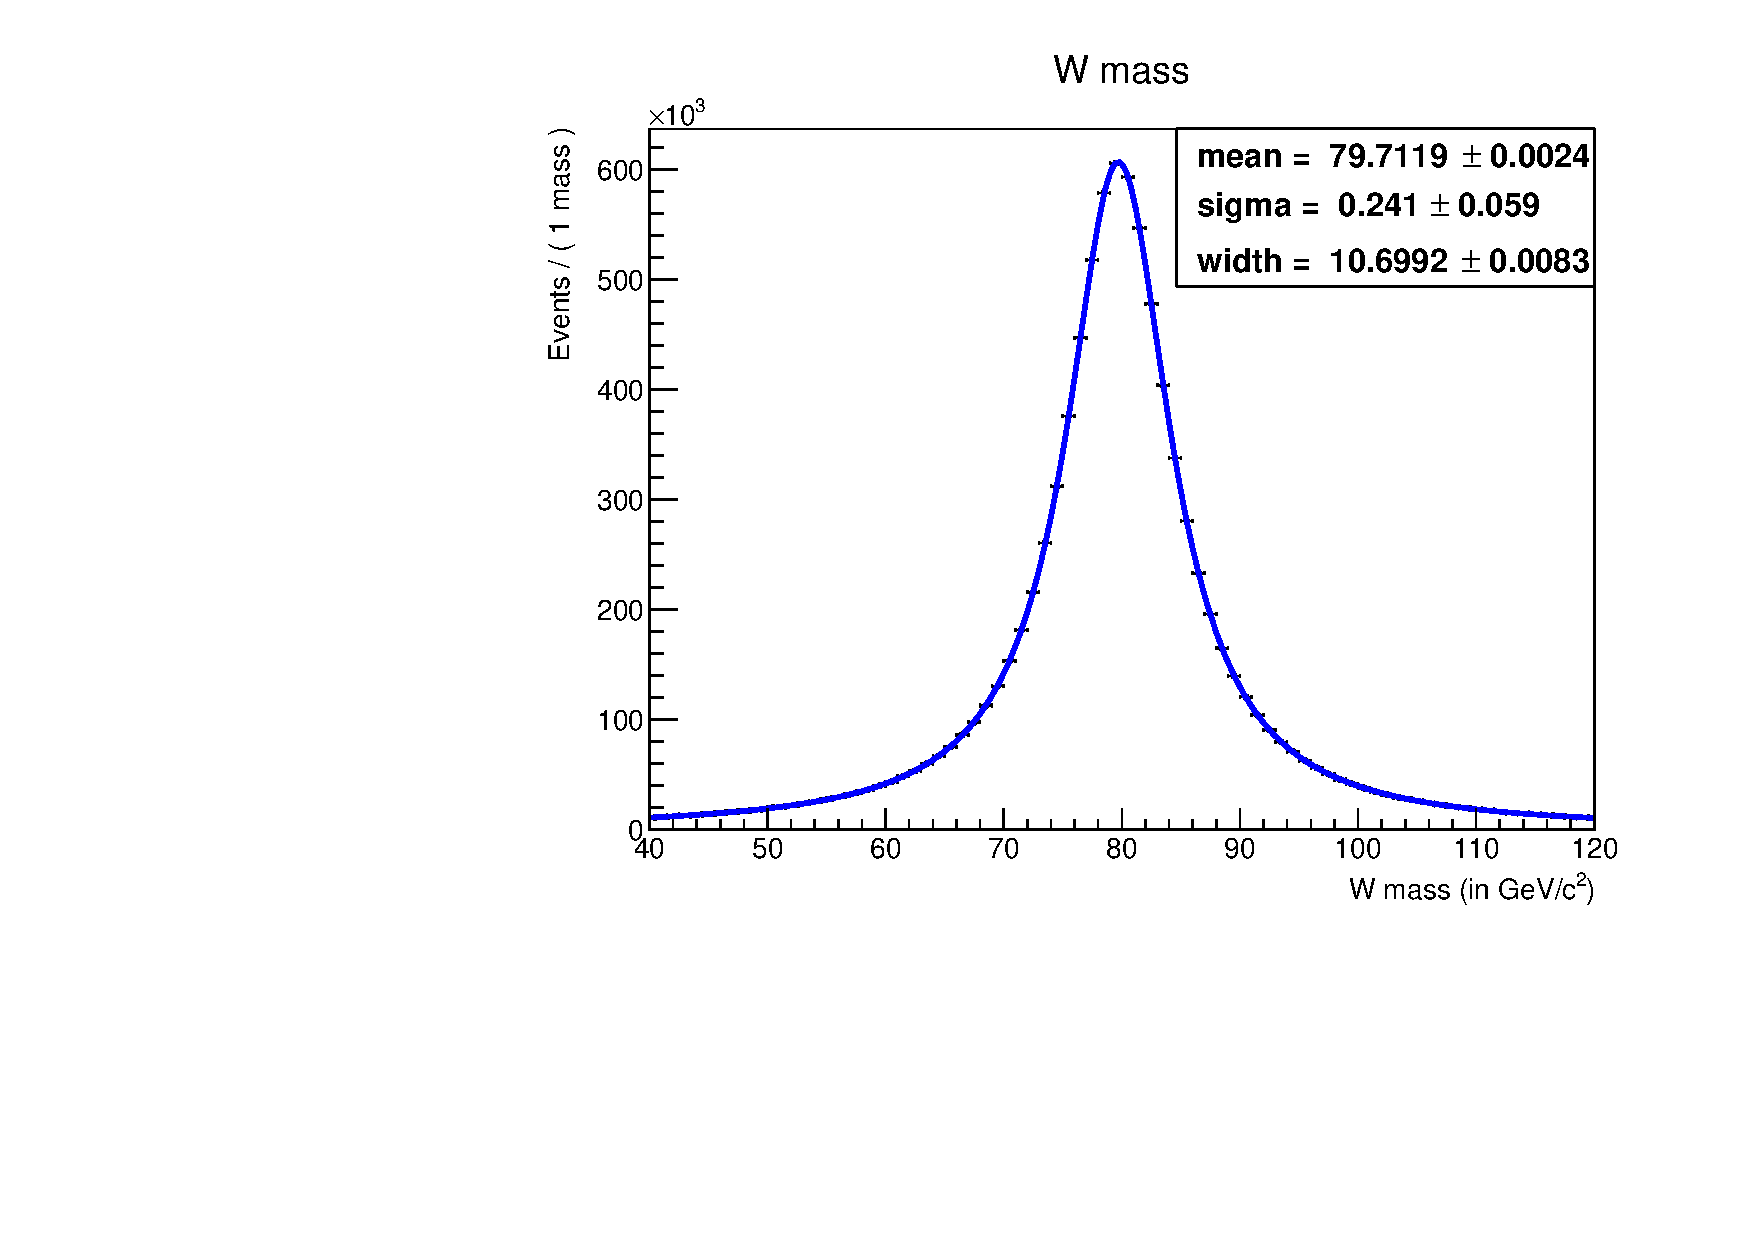
\includegraphics[width=0.99\textwidth]{Wtoyfit.pdf} % second figure itself
     
     \end{minipage}\\
     \caption{ The left distribution shows the (-0.8,+0.3) W mass distribution for all signal after selection cuts. The fit results in the Voigtian parameters $M_W = 79.7074$, width $\Gamma_W = 10.6972$ and $\sigma_W = 4.847e-7$ with Monte Carlo statistics scaled up to 1600 $\text{fb}^{-1}$. The right distribution shows the refit with 9.36M W's generated according to the fitted model.}
\label{fig:badfit}


\end{figure}


